\documentclass[twoside]{book}

% Packages required by doxygen
\usepackage{fixltx2e}
\usepackage{calc}
\usepackage{doxygen}
\usepackage[export]{adjustbox} % also loads graphicx
\usepackage{graphicx}
\usepackage[utf8]{inputenc}
\usepackage{makeidx}
\usepackage{multicol}
\usepackage{multirow}
\PassOptionsToPackage{warn}{textcomp}
\usepackage{textcomp}
\usepackage[nointegrals]{wasysym}
\usepackage[table]{xcolor}

% Font selection
\usepackage[T1]{fontenc}
\usepackage[scaled=.90]{helvet}
\usepackage{courier}
\usepackage{amssymb}
\usepackage{sectsty}
\renewcommand{\familydefault}{\sfdefault}
\allsectionsfont{%
  \fontseries{bc}\selectfont%
  \color{darkgray}%
}
\renewcommand{\DoxyLabelFont}{%
  \fontseries{bc}\selectfont%
  \color{darkgray}%
}
\newcommand{\+}{\discretionary{\mbox{\scriptsize$\hookleftarrow$}}{}{}}

% Page & text layout
\usepackage{geometry}
\geometry{%
  a4paper,%
  top=2.5cm,%
  bottom=2.5cm,%
  left=2.5cm,%
  right=2.5cm%
}
\tolerance=750
\hfuzz=15pt
\hbadness=750
\setlength{\emergencystretch}{15pt}
\setlength{\parindent}{0cm}
\setlength{\parskip}{3ex plus 2ex minus 2ex}
\makeatletter
\renewcommand{\paragraph}{%
  \@startsection{paragraph}{4}{0ex}{-1.0ex}{1.0ex}{%
    \normalfont\normalsize\bfseries\SS@parafont%
  }%
}
\renewcommand{\subparagraph}{%
  \@startsection{subparagraph}{5}{0ex}{-1.0ex}{1.0ex}{%
    \normalfont\normalsize\bfseries\SS@subparafont%
  }%
}
\makeatother

% Headers & footers
\usepackage{fancyhdr}
\pagestyle{fancyplain}
\fancyhead[LE]{\fancyplain{}{\bfseries\thepage}}
\fancyhead[CE]{\fancyplain{}{}}
\fancyhead[RE]{\fancyplain{}{\bfseries\leftmark}}
\fancyhead[LO]{\fancyplain{}{\bfseries\rightmark}}
\fancyhead[CO]{\fancyplain{}{}}
\fancyhead[RO]{\fancyplain{}{\bfseries\thepage}}
\fancyfoot[LE]{\fancyplain{}{}}
\fancyfoot[CE]{\fancyplain{}{}}
\fancyfoot[RE]{\fancyplain{}{\bfseries\scriptsize Generated by Doxygen }}
\fancyfoot[LO]{\fancyplain{}{\bfseries\scriptsize Generated by Doxygen }}
\fancyfoot[CO]{\fancyplain{}{}}
\fancyfoot[RO]{\fancyplain{}{}}
\renewcommand{\footrulewidth}{0.4pt}
\renewcommand{\chaptermark}[1]{%
  \markboth{#1}{}%
}
\renewcommand{\sectionmark}[1]{%
  \markright{\thesection\ #1}%
}

% Indices & bibliography
\usepackage{natbib}
\usepackage[titles]{tocloft}
\setcounter{tocdepth}{3}
\setcounter{secnumdepth}{5}
\makeindex

% Hyperlinks (required, but should be loaded last)
\usepackage{ifpdf}
\ifpdf
  \usepackage[pdftex,pagebackref=true]{hyperref}
\else
  \usepackage[ps2pdf,pagebackref=true]{hyperref}
\fi
\hypersetup{%
  colorlinks=true,%
  linkcolor=blue,%
  citecolor=blue,%
  unicode%
}

% Custom commands
\newcommand{\clearemptydoublepage}{%
  \newpage{\pagestyle{empty}\cleardoublepage}%
}

\usepackage{caption}
\captionsetup{labelsep=space,justification=centering,font={bf},singlelinecheck=off,skip=4pt,position=top}

%===== C O N T E N T S =====

\begin{document}

% Titlepage & ToC
\hypersetup{pageanchor=false,
             bookmarksnumbered=true,
             pdfencoding=unicode
            }
\pagenumbering{alph}
\begin{titlepage}
\vspace*{7cm}
\begin{center}%
{\Large The Octantis project }\\
\vspace*{1cm}
{\large Generated by Doxygen 1.8.13}\\
\end{center}
\end{titlepage}
\clearemptydoublepage
\pagenumbering{roman}
\tableofcontents
\clearemptydoublepage
\pagenumbering{arabic}
\hypersetup{pageanchor=true}

%--- Begin generated contents ---
\chapter{The Octantis Project}
\label{index}\hypertarget{index}{}\subsubsection*{An High-\/\+Level Explorer for Logic-\/in-\/\+Memory architectures.}

\subsection*{Licence }

© Andrea Marchesin 2020 (\href{mailto:andrea.marchesin@studenti.polito.it}{\tt andrea.\+marchesin@studenti.\+polito.\+it}) for Politecnico di Torino





\subsection*{Instructions for the compilation of the project -\/ Warning\+: It may require many Gb of free memory! }


\begin{DoxyEnumerate}
\item Create a \char`\"{}build\char`\"{} folder, outside the Git repository
\item Enter the newly created folder and execute the following commands\+: ``` cmake -\/G \textquotesingle{}Unix Makefiles\textquotesingle{} ../\+The-\/\+Octantis-\/project/llvm -\/\+D\+L\+L\+V\+M\+\_\+\+U\+S\+E\+\_\+\+L\+I\+N\+K\+ER=gold -\/\+D\+C\+M\+A\+K\+E\+\_\+\+B\+U\+I\+L\+D\+\_\+\+T\+Y\+PE=Release make ```
\end{DoxyEnumerate}

$\ast$\+N\+O\+T\+ES\+: The serial compilation is extremely slow, so the following code is suggested\+: {\ttfamily make -\/j \#\+Nuber of available C\+P\+Us\#} 



After the building of the project, all the passes developed can be tested. More detail will be released in the future version of the project.





\subsection*{A brief introduction to the project }

Today, one of the problems the scientific community is called upon to tackle is the well-\/known {\itshape von Neumann bottleneck}. The latter involves two crucial elements in a digital electronic system, the C\+PU and the memory, which suffer from a limitation in bandwidth they exchange information with. The latency which characterizes the transmission of the data between these electronic devices predominantly depends on\+:
\begin{DoxyItemize}
\item The strict physical parameters which describe the behavior of the {\itshape interconnections} linking the memory and the processing unit.
\item The diminished $\ast$performance of the memories $\ast$themselves compared to that of the processing unit.
\end{DoxyItemize}

Among the various solutions under study, in the recent years the V\+L\+SI Laboratory of Politecnico di Torino has proposed the concept of {\itshape Logic-\/\+In-\/\+Memory (L\+IM)}\+: a memory device which embeds simple computational elements between the different cells, overall arranging a distributed processing system. The key idea consists in reducing access to the memory for the C\+PU, implementing a precomputation of raw data within the same memory. The C\+PU is left only with the task of performing the more complex operations on that pre-\/processed information. Different architectures have been proposed during the years and since 2019 the research group decided to go beyond the realization of specific case of study. In this context, {\itshape D\+Ex\+I\+MA} was born as a “beta version” of a software tool able to characterize generic Logic-\/\+In-\/\+Memory architectures. The information which the program can provide refers to space occupation, maximum performance and static and dynamic power consumption. In order to do that, D\+Ex\+I\+MA relies on a detailed library of components which are constantly updated. Today attention is given on the definition of C-\/\+M\+OS components, but above C-\/\+M\+OS solutions are already starting to be taken into consideration, like {\itshape Nano Magnetic Logic} and {\itshape perpendicular Nano Magnetic Logic}.

The thesis work has been inserted into this context with the introduction of {\itshape Octantis}, a software designed form scratch useful for the exploration of L\+IM architectures. By its nature it is a flexible solution to analyze an input algorithm described in standard C language and to identify which L\+IM architecture would implement it better. Only a subset of operations in the input C code is allowed and the algorithm so described must be accompanied by a configuration file, in which the L\+IM designer has to impose the constraints that Octantis considers to model the architecture in accordance with them. At the output of the program the D\+Ex\+I\+MA configuration files are provided, in order to enable the simulator engine to perform the related analysis. Octantis and D\+Ex\+I\+MA merge in a unique software of first approach in the design phase, which allows the designer to get an idea of what the benefits might be in the implementation of a specific algorithm through a Logic-\/\+In-\/\+Memory structure. The term of comparison is the execution of the same algorithm in a traditional microprocessor system.

The Octantis’ project considers the {\itshape L\+L\+VM compiler infrastructure} to realize the whole process of translation from C-\/code to D\+Ex\+I\+MA input files. The L\+L\+VM framework provides libraries useful to optimize and generate a code for a target architecture starting from an input source. It is distributed under an opensource license, which allows a free customization of each of its components. In the panorama of C compilers, the choice fell on L\+L\+VM, to the detriment of the tools provided by the competitor {\itshape G\+N\+U-\/\+G\+CC}, considering specially the flexibility of the former infrastructure, which can count on a more active community of developers and richer technical documentations.



The whole project has been designed so as to guarantee the {\itshape modularity} and the {\itshape maintenance} of the code. For what concerns the maintenance, a detailed documentation is provided together with Octantis in order to prepare the designer to work on it in a short time. The modularity is then guaranteed to allow the same developers to extend the capability of the tool during time.

At the state of art, many other features can be introduced. A future work goal could be the analysis of a generic C source code to define, directly when Octantis starts, which parts of the whole algorithm could benefit of a L\+IM implementation and which would not. In this way, only a portion of the source code would be mapped on a L\+IM architecture while the remaining part could be rearranged to be provided to a generic processor back-\/end. This new version of Octantis would be able to collect information on how a more complex system, composed by a L\+I\+M-\/\+Memory associated to a modern processor, would behave. Moreover, considering the further developments on the D\+Ex\+I\+MA library, also new input operations could be mapped in a more efficient way. Therefore, it could be useful to extend the capabilities of Octantis itself.

These are few of the possible future works which could be realized around Octantis and, in general, the coupled {\itshape Octantis-\/\+D\+Ex\+I\+MA}.

In conclusion, the hope is to have realized an instrument capable of giving light to the many Logic-\/\+In-\/\+Memory researches that have been carried out so far by the researchers of the V\+L\+SI Laboratory. Octantis aims to be a {\itshape valid guide} during the exploratory phase of L\+IM architectures, a promising solution for how electronics could evolve in the coming years. 

 
\chapter{Namespace Index}
\section{Namespace List}
Here is a list of all namespaces with brief descriptions\+:\begin{DoxyCompactList}
\item\contentsline{section}{\hyperlink{namespaceoctantis}{octantis} }{\pageref{namespaceoctantis}}{}
\end{DoxyCompactList}

\chapter{Hierarchical Index}
\section{Class Hierarchy}
This inheritance list is sorted roughly, but not completely, alphabetically\+:\begin{DoxyCompactList}
\item \contentsline{section}{octantis\+:\+:Instruction\+Table\+:\+:allocated\+Data}{\pageref{structoctantis_1_1InstructionTable_1_1allocatedData}}{}
\item \contentsline{section}{octantis\+:\+:Finite\+State\+Machine}{\pageref{classoctantis_1_1FiniteStateMachine}}{}
\item Function\+Pass\begin{DoxyCompactList}
\item \contentsline{section}{octantis\+:\+:Octantis\+Pass}{\pageref{structoctantis_1_1OctantisPass}}{}
\end{DoxyCompactList}
\item \contentsline{section}{octantis\+:\+:Instruction\+Table\+:\+:instruction\+Data}{\pageref{structoctantis_1_1InstructionTable_1_1instructionData}}{}
\item \contentsline{section}{octantis\+:\+:Instruction\+Table}{\pageref{classoctantis_1_1InstructionTable}}{}
\item \contentsline{section}{octantis\+:\+:Li\+M\+Array}{\pageref{classoctantis_1_1LiMArray}}{}
\item \contentsline{section}{octantis\+:\+:Li\+M\+Compiler}{\pageref{classoctantis_1_1LiMCompiler}}{}
\item \contentsline{section}{octantis\+:\+:Li\+M\+Array\+:\+:Li\+M\+Row}{\pageref{structoctantis_1_1LiMArray_1_1LiMRow}}{}
\item \contentsline{section}{octantis\+:\+:Print\+Dex\+File}{\pageref{classoctantis_1_1PrintDexFile}}{}
\item \contentsline{section}{octantis\+:\+:Scheduling\+A\+S\+AP}{\pageref{classoctantis_1_1SchedulingASAP}}{}
\end{DoxyCompactList}

\chapter{Class Index}
\section{Class List}
Here are the classes, structs, unions and interfaces with brief descriptions\+:\begin{DoxyCompactList}
\item\contentsline{section}{\hyperlink{structoctantis_1_1InstructionTable_1_1allocatedData}{octantis\+::\+Instruction\+Table\+::allocated\+Data} }{\pageref{structoctantis_1_1InstructionTable_1_1allocatedData}}{}
\item\contentsline{section}{\hyperlink{classoctantis_1_1FiniteStateMachine}{octantis\+::\+Finite\+State\+Machine} \\*Class useful for the definition of the F\+SM of the algorithm }{\pageref{classoctantis_1_1FiniteStateMachine}}{}
\item\contentsline{section}{\hyperlink{structoctantis_1_1InstructionTable_1_1instructionData}{octantis\+::\+Instruction\+Table\+::instruction\+Data} \\*Structure useful to store the information related to each L\+L\+VM instruction }{\pageref{structoctantis_1_1InstructionTable_1_1instructionData}}{}
\item\contentsline{section}{\hyperlink{classoctantis_1_1InstructionTable}{octantis\+::\+Instruction\+Table} \\*Class useful to store the instructions that will be scheduled on the LiM architecture }{\pageref{classoctantis_1_1InstructionTable}}{}
\item\contentsline{section}{\hyperlink{classoctantis_1_1LiMArray}{octantis\+::\+Li\+M\+Array} \\*Class implementing the necessary structures to model the LiM Unit }{\pageref{classoctantis_1_1LiMArray}}{}
\item\contentsline{section}{\hyperlink{classoctantis_1_1LiMCompiler}{octantis\+::\+Li\+M\+Compiler} \\*Class class useful for the generation of a LiM object }{\pageref{classoctantis_1_1LiMCompiler}}{}
\item\contentsline{section}{\hyperlink{structoctantis_1_1LiMArray_1_1LiMRow}{octantis\+::\+Li\+M\+Array\+::\+Li\+M\+Row} \\*Lim row description }{\pageref{structoctantis_1_1LiMArray_1_1LiMRow}}{}
\item\contentsline{section}{\hyperlink{structoctantis_1_1OctantisPass}{octantis\+::\+Octantis\+Pass} }{\pageref{structoctantis_1_1OctantisPass}}{}
\item\contentsline{section}{\hyperlink{classoctantis_1_1PrintDexFile}{octantis\+::\+Print\+Dex\+File} \\*Class class useful for the definition of Dexima\textquotesingle{}s configuration file (.dex) }{\pageref{classoctantis_1_1PrintDexFile}}{}
\item\contentsline{section}{\hyperlink{classoctantis_1_1SchedulingASAP}{octantis\+::\+Scheduling\+A\+S\+AP} \\*Class useful for the implementation of the A\+S\+AP Scheduling algorithm }{\pageref{classoctantis_1_1SchedulingASAP}}{}
\end{DoxyCompactList}

\chapter{File Index}
\section{File List}
Here is a list of all files with brief descriptions\+:\begin{DoxyCompactList}
\item\contentsline{section}{/home/andrea/\+Documenti/\+Octantis\+V1.\+0/\+The-\/\+Octantis-\/project/llvm/lib/\+Transforms/\+Octantis/\hyperlink{AdditionalLogicPorts_8cpp}{Additional\+Logic\+Ports.\+cpp} }{\pageref{AdditionalLogicPorts_8cpp}}{}
\item\contentsline{section}{/home/andrea/\+Documenti/\+Octantis\+V1.\+0/\+The-\/\+Octantis-\/project/llvm/lib/\+Transforms/\+Octantis/\hyperlink{AdditionalLogicPorts_8h}{Additional\+Logic\+Ports.\+h} }{\pageref{AdditionalLogicPorts_8h}}{}
\item\contentsline{section}{/home/andrea/\+Documenti/\+Octantis\+V1.\+0/\+The-\/\+Octantis-\/project/llvm/lib/\+Transforms/\+Octantis/\hyperlink{FiniteStateMachine_8cpp}{Finite\+State\+Machine.\+cpp} }{\pageref{FiniteStateMachine_8cpp}}{}
\item\contentsline{section}{/home/andrea/\+Documenti/\+Octantis\+V1.\+0/\+The-\/\+Octantis-\/project/llvm/lib/\+Transforms/\+Octantis/\hyperlink{FiniteStateMachine_8h}{Finite\+State\+Machine.\+h} }{\pageref{FiniteStateMachine_8h}}{}
\item\contentsline{section}{/home/andrea/\+Documenti/\+Octantis\+V1.\+0/\+The-\/\+Octantis-\/project/llvm/lib/\+Transforms/\+Octantis/\hyperlink{InstructionTable_8cpp}{Instruction\+Table.\+cpp} }{\pageref{InstructionTable_8cpp}}{}
\item\contentsline{section}{/home/andrea/\+Documenti/\+Octantis\+V1.\+0/\+The-\/\+Octantis-\/project/llvm/lib/\+Transforms/\+Octantis/\hyperlink{InstructionTable_8h}{Instruction\+Table.\+h} }{\pageref{InstructionTable_8h}}{}
\item\contentsline{section}{/home/andrea/\+Documenti/\+Octantis\+V1.\+0/\+The-\/\+Octantis-\/project/llvm/lib/\+Transforms/\+Octantis/\hyperlink{LiMArray_8cpp}{Li\+M\+Array.\+cpp} }{\pageref{LiMArray_8cpp}}{}
\item\contentsline{section}{/home/andrea/\+Documenti/\+Octantis\+V1.\+0/\+The-\/\+Octantis-\/project/llvm/lib/\+Transforms/\+Octantis/\hyperlink{LiMArray_8h}{Li\+M\+Array.\+h} }{\pageref{LiMArray_8h}}{}
\item\contentsline{section}{/home/andrea/\+Documenti/\+Octantis\+V1.\+0/\+The-\/\+Octantis-\/project/llvm/lib/\+Transforms/\+Octantis/\hyperlink{LiMCompiler_8cpp}{Li\+M\+Compiler.\+cpp} }{\pageref{LiMCompiler_8cpp}}{}
\item\contentsline{section}{/home/andrea/\+Documenti/\+Octantis\+V1.\+0/\+The-\/\+Octantis-\/project/llvm/lib/\+Transforms/\+Octantis/\hyperlink{LiMCompiler_8h}{Li\+M\+Compiler.\+h} }{\pageref{LiMCompiler_8h}}{}
\item\contentsline{section}{/home/andrea/\+Documenti/\+Octantis\+V1.\+0/\+The-\/\+Octantis-\/project/llvm/lib/\+Transforms/\+Octantis/\hyperlink{OctantisPass_8cpp}{Octantis\+Pass.\+cpp} }{\pageref{OctantisPass_8cpp}}{}
\item\contentsline{section}{/home/andrea/\+Documenti/\+Octantis\+V1.\+0/\+The-\/\+Octantis-\/project/llvm/lib/\+Transforms/\+Octantis/\hyperlink{OperationsImplemented_8h}{Operations\+Implemented.\+h} }{\pageref{OperationsImplemented_8h}}{}
\item\contentsline{section}{/home/andrea/\+Documenti/\+Octantis\+V1.\+0/\+The-\/\+Octantis-\/project/llvm/lib/\+Transforms/\+Octantis/\hyperlink{PrintDexFile_8cpp}{Print\+Dex\+File.\+cpp} }{\pageref{PrintDexFile_8cpp}}{}
\item\contentsline{section}{/home/andrea/\+Documenti/\+Octantis\+V1.\+0/\+The-\/\+Octantis-\/project/llvm/lib/\+Transforms/\+Octantis/\hyperlink{PrintDexFile_8h}{Print\+Dex\+File.\+h} }{\pageref{PrintDexFile_8h}}{}
\item\contentsline{section}{/home/andrea/\+Documenti/\+Octantis\+V1.\+0/\+The-\/\+Octantis-\/project/llvm/lib/\+Transforms/\+Octantis/\hyperlink{SchedulingASAP_8cpp}{Scheduling\+A\+S\+A\+P.\+cpp} }{\pageref{SchedulingASAP_8cpp}}{}
\item\contentsline{section}{/home/andrea/\+Documenti/\+Octantis\+V1.\+0/\+The-\/\+Octantis-\/project/llvm/lib/\+Transforms/\+Octantis/\hyperlink{SchedulingASAP_8h}{Scheduling\+A\+S\+A\+P.\+h} }{\pageref{SchedulingASAP_8h}}{}
\end{DoxyCompactList}

\chapter{Namespace Documentation}
\hypertarget{namespaceoctantis}{}\section{octantis Namespace Reference}
\label{namespaceoctantis}\index{octantis@{octantis}}
\subsection*{Classes}
\begin{DoxyCompactItemize}
\item 
class \hyperlink{classoctantis_1_1FiniteStateMachine}{Finite\+State\+Machine}
\begin{DoxyCompactList}\small\item\em Class useful for the definition of the F\+SM of the algorithm. \end{DoxyCompactList}\item 
class \hyperlink{classoctantis_1_1InstructionTable}{Instruction\+Table}
\begin{DoxyCompactList}\small\item\em Class useful to store the instructions that will be scheduled on the LiM architecture. \end{DoxyCompactList}\item 
class \hyperlink{classoctantis_1_1LiMArray}{Li\+M\+Array}
\begin{DoxyCompactList}\small\item\em Class implementing the necessary structures to model the LiM Unit. \end{DoxyCompactList}\item 
class \hyperlink{classoctantis_1_1LiMCompiler}{Li\+M\+Compiler}
\begin{DoxyCompactList}\small\item\em Class class useful for the generation of a LiM object. \end{DoxyCompactList}\item 
struct \hyperlink{structoctantis_1_1OctantisPass}{Octantis\+Pass}
\item 
class \hyperlink{classoctantis_1_1PrintDexFile}{Print\+Dex\+File}
\begin{DoxyCompactList}\small\item\em Class class useful for the definition of Dexima\textquotesingle{}s configuration file (.dex). \end{DoxyCompactList}\item 
class \hyperlink{classoctantis_1_1SchedulingASAP}{Scheduling\+A\+S\+AP}
\begin{DoxyCompactList}\small\item\em Class useful for the implementation of the A\+S\+AP Scheduling algorithm. \end{DoxyCompactList}\end{DoxyCompactItemize}
\subsection*{Variables}
\begin{DoxyCompactItemize}
\item 
const std\+::map$<$ std\+::string, std\+::string $>$ \hyperlink{namespaceoctantis_a49f0001417908900d6959ac7a8037ebd}{Lim\+Operations}
\item 
const std\+::set$<$ std\+::string $>$ \hyperlink{namespaceoctantis_adec74f4b9921d5c7eecef4f9174c3510}{Periperal\+Operations}
\end{DoxyCompactItemize}


\subsection{Variable Documentation}
\mbox{\Hypertarget{namespaceoctantis_a49f0001417908900d6959ac7a8037ebd}\label{namespaceoctantis_a49f0001417908900d6959ac7a8037ebd}} 
\index{octantis@{octantis}!Lim\+Operations@{Lim\+Operations}}
\index{Lim\+Operations@{Lim\+Operations}!octantis@{octantis}}
\subsubsection{\texorpdfstring{Lim\+Operations}{LimOperations}}
{\footnotesize\ttfamily const std\+::map$<$std\+::string, std\+::string$>$ octantis\+::\+Lim\+Operations}

{\bfseries Initial value\+:}
\begin{DoxyCode}
= \{
    \{\textcolor{stringliteral}{"load"}, \textcolor{stringliteral}{"null"}\},
    \{\textcolor{stringliteral}{"add"}, \textcolor{stringliteral}{"arith"}\},
    \{\textcolor{stringliteral}{"sub"}, \textcolor{stringliteral}{"arith"}\},
    \{\textcolor{stringliteral}{"and"}, \textcolor{stringliteral}{"bitwise"}\},
    \{\textcolor{stringliteral}{"nand"}, \textcolor{stringliteral}{"bitwise"}\},
    \{\textcolor{stringliteral}{"or"}, \textcolor{stringliteral}{"bitwise"}\},
    \{\textcolor{stringliteral}{"xor"}, \textcolor{stringliteral}{"bitwise"}\}
\}
\end{DoxyCode}
\mbox{\Hypertarget{namespaceoctantis_adec74f4b9921d5c7eecef4f9174c3510}\label{namespaceoctantis_adec74f4b9921d5c7eecef4f9174c3510}} 
\index{octantis@{octantis}!Periperal\+Operations@{Periperal\+Operations}}
\index{Periperal\+Operations@{Periperal\+Operations}!octantis@{octantis}}
\subsubsection{\texorpdfstring{Periperal\+Operations}{PeriperalOperations}}
{\footnotesize\ttfamily const std\+::set$<$std\+::string$>$ octantis\+::\+Periperal\+Operations}

{\bfseries Initial value\+:}
\begin{DoxyCode}
= \{
    \textcolor{stringliteral}{"mux"},
    \textcolor{stringliteral}{"popcount"},
    \textcolor{stringliteral}{"upcount"}
\}
\end{DoxyCode}

\chapter{Class Documentation}
\hypertarget{classoctantis_1_1AdditionalLogicPorts}{}\section{octantis\+:\+:Additional\+Logic\+Ports Class Reference}
\label{classoctantis_1_1AdditionalLogicPorts}\index{octantis\+::\+Additional\+Logic\+Ports@{octantis\+::\+Additional\+Logic\+Ports}}


{\ttfamily \#include $<$Additional\+Logic\+Ports.\+h$>$}

\subsection*{Public Member Functions}
\begin{DoxyCompactItemize}
\item 
\hyperlink{classoctantis_1_1AdditionalLogicPorts_a0c1279363e919e4d82caddf4a486f56e}{Additional\+Logic\+Ports} ()
\item 
std\+::string \hyperlink{classoctantis_1_1AdditionalLogicPorts_a375d3e65187034c5c2fdf80bf22d49d7}{get\+Negative\+Logic} (std\+::string logic)
\begin{DoxyCompactList}\small\item\em It returns the corresponding negative logic. \end{DoxyCompactList}\end{DoxyCompactItemize}


\subsection{Detailed Description}
It extends the L\+L\+VM IR language introducing all the logic ports available in the R\+TL design. 

Definition at line 24 of file Additional\+Logic\+Ports.\+h.



\subsection{Constructor \& Destructor Documentation}
\mbox{\Hypertarget{classoctantis_1_1AdditionalLogicPorts_a0c1279363e919e4d82caddf4a486f56e}\label{classoctantis_1_1AdditionalLogicPorts_a0c1279363e919e4d82caddf4a486f56e}} 
\index{octantis\+::\+Additional\+Logic\+Ports@{octantis\+::\+Additional\+Logic\+Ports}!Additional\+Logic\+Ports@{Additional\+Logic\+Ports}}
\index{Additional\+Logic\+Ports@{Additional\+Logic\+Ports}!octantis\+::\+Additional\+Logic\+Ports@{octantis\+::\+Additional\+Logic\+Ports}}
\subsubsection{\texorpdfstring{Additional\+Logic\+Ports()}{AdditionalLogicPorts()}}
{\footnotesize\ttfamily Additional\+Logic\+Ports\+::\+Additional\+Logic\+Ports (\begin{DoxyParamCaption}{ }\end{DoxyParamCaption})}



Definition at line 18 of file Additional\+Logic\+Ports.\+cpp.



\subsection{Member Function Documentation}
\mbox{\Hypertarget{classoctantis_1_1AdditionalLogicPorts_a375d3e65187034c5c2fdf80bf22d49d7}\label{classoctantis_1_1AdditionalLogicPorts_a375d3e65187034c5c2fdf80bf22d49d7}} 
\index{octantis\+::\+Additional\+Logic\+Ports@{octantis\+::\+Additional\+Logic\+Ports}!get\+Negative\+Logic@{get\+Negative\+Logic}}
\index{get\+Negative\+Logic@{get\+Negative\+Logic}!octantis\+::\+Additional\+Logic\+Ports@{octantis\+::\+Additional\+Logic\+Ports}}
\subsubsection{\texorpdfstring{get\+Negative\+Logic()}{getNegativeLogic()}}
{\footnotesize\ttfamily std\+::string Additional\+Logic\+Ports\+::get\+Negative\+Logic (\begin{DoxyParamCaption}\item[{std\+::string}]{logic }\end{DoxyParamCaption})}



It returns the corresponding negative logic. 



Definition at line 24 of file Additional\+Logic\+Ports.\+cpp.



The documentation for this class was generated from the following files\+:\begin{DoxyCompactItemize}
\item 
/home/andrea/\+Documenti/\+Octantis\+V1.\+0/\+The-\/\+Octantis-\/project/llvm/lib/\+Transforms/\+Octantis/\hyperlink{AdditionalLogicPorts_8h}{Additional\+Logic\+Ports.\+h}\item 
/home/andrea/\+Documenti/\+Octantis\+V1.\+0/\+The-\/\+Octantis-\/project/llvm/lib/\+Transforms/\+Octantis/\hyperlink{AdditionalLogicPorts_8cpp}{Additional\+Logic\+Ports.\+cpp}\end{DoxyCompactItemize}

\hypertarget{structoctantis_1_1InstructionTable_1_1allocatedData}{}\section{octantis\+:\+:Instruction\+Table\+:\+:allocated\+Data Struct Reference}
\label{structoctantis_1_1InstructionTable_1_1allocatedData}\index{octantis\+::\+Instruction\+Table\+::allocated\+Data@{octantis\+::\+Instruction\+Table\+::allocated\+Data}}


{\ttfamily \#include $<$Instruction\+Table.\+h$>$}

\subsection*{Public Attributes}
\begin{DoxyCompactItemize}
\item 
int \hyperlink{structoctantis_1_1InstructionTable_1_1allocatedData_a93134066380dd21870cb0ae4e427e274}{alloc\+Time}
\item 
bool \hyperlink{structoctantis_1_1InstructionTable_1_1allocatedData_aa1655d3d2df0738a28ed8f722151f347}{valid}
\end{DoxyCompactItemize}


\subsection{Detailed Description}
Allocated data\+: they are typically inside the stack, so outside the memory. The struct is useful to support the identification if one of these data has been modified. 

\subsection{Member Data Documentation}
\mbox{\Hypertarget{structoctantis_1_1InstructionTable_1_1allocatedData_a93134066380dd21870cb0ae4e427e274}\label{structoctantis_1_1InstructionTable_1_1allocatedData_a93134066380dd21870cb0ae4e427e274}} 
\index{octantis\+::\+Instruction\+Table\+::allocated\+Data@{octantis\+::\+Instruction\+Table\+::allocated\+Data}!alloc\+Time@{alloc\+Time}}
\index{alloc\+Time@{alloc\+Time}!octantis\+::\+Instruction\+Table\+::allocated\+Data@{octantis\+::\+Instruction\+Table\+::allocated\+Data}}
\subsubsection{\texorpdfstring{alloc\+Time}{allocTime}}
{\footnotesize\ttfamily int octantis\+::\+Instruction\+Table\+::allocated\+Data\+::alloc\+Time}

\mbox{\Hypertarget{structoctantis_1_1InstructionTable_1_1allocatedData_aa1655d3d2df0738a28ed8f722151f347}\label{structoctantis_1_1InstructionTable_1_1allocatedData_aa1655d3d2df0738a28ed8f722151f347}} 
\index{octantis\+::\+Instruction\+Table\+::allocated\+Data@{octantis\+::\+Instruction\+Table\+::allocated\+Data}!valid@{valid}}
\index{valid@{valid}!octantis\+::\+Instruction\+Table\+::allocated\+Data@{octantis\+::\+Instruction\+Table\+::allocated\+Data}}
\subsubsection{\texorpdfstring{valid}{valid}}
{\footnotesize\ttfamily bool octantis\+::\+Instruction\+Table\+::allocated\+Data\+::valid}



The documentation for this struct was generated from the following file\+:\begin{DoxyCompactItemize}
\item 
/home/andrea/\+Documenti/\+Octantis\+V1.\+0/\+The-\/\+Octantis-\/project/llvm/lib/\+Transforms/\+Octantis/\hyperlink{InstructionTable_8h}{Instruction\+Table.\+h}\end{DoxyCompactItemize}

\hypertarget{classoctantis_1_1FiniteStateMachine}{}\section{octantis\+:\+:Finite\+State\+Machine Class Reference}
\label{classoctantis_1_1FiniteStateMachine}\index{octantis\+::\+Finite\+State\+Machine@{octantis\+::\+Finite\+State\+Machine}}


Class useful for the definition of the F\+SM of the algorithm.  




{\ttfamily \#include $<$Finite\+State\+Machine.\+h$>$}

\subsection*{Public Member Functions}
\begin{DoxyCompactItemize}
\item 
\hyperlink{classoctantis_1_1FiniteStateMachine_a7f4b2e43939afa064ee2d8232ad9634e}{Finite\+State\+Machine} ()
\item 
void \hyperlink{classoctantis_1_1FiniteStateMachine_a598e2f7c88a6ad25475edd96229eda21}{add\+New\+Instruction} (int \&time, int $\ast$const \&operand)
\begin{DoxyCompactList}\small\item\em Function to allocate a new operation in a precise time. \end{DoxyCompactList}\item 
int \hyperlink{classoctantis_1_1FiniteStateMachine_a14a05f7b6fde7318d3c7b3c8e7d1a504}{get\+F\+S\+M\+Size} ()
\begin{DoxyCompactList}\small\item\em Function to get the size of the F\+SM. \end{DoxyCompactList}\item 
void \hyperlink{classoctantis_1_1FiniteStateMachine_a6f65084e2058b3eb5a76bcddea769839}{print\+F\+SM} ()
\end{DoxyCompactItemize}
\subsection*{Public Attributes}
\begin{DoxyCompactItemize}
\item 
std\+::map$<$ int, std\+::list$<$ int $\ast$ $>$ $>$ \hyperlink{classoctantis_1_1FiniteStateMachine_ab794f5f9bd9e5ca27f6834a644ed62ef}{F\+SM}
\end{DoxyCompactItemize}


\subsection{Detailed Description}
Class useful for the definition of the F\+SM of the algorithm. 

Definition at line 21 of file Finite\+State\+Machine.\+h.



\subsection{Constructor \& Destructor Documentation}
\mbox{\Hypertarget{classoctantis_1_1FiniteStateMachine_a7f4b2e43939afa064ee2d8232ad9634e}\label{classoctantis_1_1FiniteStateMachine_a7f4b2e43939afa064ee2d8232ad9634e}} 
\index{octantis\+::\+Finite\+State\+Machine@{octantis\+::\+Finite\+State\+Machine}!Finite\+State\+Machine@{Finite\+State\+Machine}}
\index{Finite\+State\+Machine@{Finite\+State\+Machine}!octantis\+::\+Finite\+State\+Machine@{octantis\+::\+Finite\+State\+Machine}}
\subsubsection{\texorpdfstring{Finite\+State\+Machine()}{FiniteStateMachine()}}
{\footnotesize\ttfamily Finite\+State\+Machine\+::\+Finite\+State\+Machine (\begin{DoxyParamCaption}{ }\end{DoxyParamCaption})}



Definition at line 17 of file Finite\+State\+Machine.\+cpp.



\subsection{Member Function Documentation}
\mbox{\Hypertarget{classoctantis_1_1FiniteStateMachine_a598e2f7c88a6ad25475edd96229eda21}\label{classoctantis_1_1FiniteStateMachine_a598e2f7c88a6ad25475edd96229eda21}} 
\index{octantis\+::\+Finite\+State\+Machine@{octantis\+::\+Finite\+State\+Machine}!add\+New\+Instruction@{add\+New\+Instruction}}
\index{add\+New\+Instruction@{add\+New\+Instruction}!octantis\+::\+Finite\+State\+Machine@{octantis\+::\+Finite\+State\+Machine}}
\subsubsection{\texorpdfstring{add\+New\+Instruction()}{addNewInstruction()}}
{\footnotesize\ttfamily void Finite\+State\+Machine\+::add\+New\+Instruction (\begin{DoxyParamCaption}\item[{int \&}]{time,  }\item[{int $\ast$const \&}]{operand }\end{DoxyParamCaption})}



Function to allocate a new operation in a precise time. 



Definition at line 23 of file Finite\+State\+Machine.\+cpp.

\mbox{\Hypertarget{classoctantis_1_1FiniteStateMachine_a14a05f7b6fde7318d3c7b3c8e7d1a504}\label{classoctantis_1_1FiniteStateMachine_a14a05f7b6fde7318d3c7b3c8e7d1a504}} 
\index{octantis\+::\+Finite\+State\+Machine@{octantis\+::\+Finite\+State\+Machine}!get\+F\+S\+M\+Size@{get\+F\+S\+M\+Size}}
\index{get\+F\+S\+M\+Size@{get\+F\+S\+M\+Size}!octantis\+::\+Finite\+State\+Machine@{octantis\+::\+Finite\+State\+Machine}}
\subsubsection{\texorpdfstring{get\+F\+S\+M\+Size()}{getFSMSize()}}
{\footnotesize\ttfamily int Finite\+State\+Machine\+::get\+F\+S\+M\+Size (\begin{DoxyParamCaption}{ }\end{DoxyParamCaption})}



Function to get the size of the F\+SM. 



Definition at line 40 of file Finite\+State\+Machine.\+cpp.

\mbox{\Hypertarget{classoctantis_1_1FiniteStateMachine_a6f65084e2058b3eb5a76bcddea769839}\label{classoctantis_1_1FiniteStateMachine_a6f65084e2058b3eb5a76bcddea769839}} 
\index{octantis\+::\+Finite\+State\+Machine@{octantis\+::\+Finite\+State\+Machine}!print\+F\+SM@{print\+F\+SM}}
\index{print\+F\+SM@{print\+F\+SM}!octantis\+::\+Finite\+State\+Machine@{octantis\+::\+Finite\+State\+Machine}}
\subsubsection{\texorpdfstring{print\+F\+S\+M()}{printFSM()}}
{\footnotesize\ttfamily void Finite\+State\+Machine\+::print\+F\+SM (\begin{DoxyParamCaption}{ }\end{DoxyParamCaption})}



Definition at line 45 of file Finite\+State\+Machine.\+cpp.



\subsection{Member Data Documentation}
\mbox{\Hypertarget{classoctantis_1_1FiniteStateMachine_ab794f5f9bd9e5ca27f6834a644ed62ef}\label{classoctantis_1_1FiniteStateMachine_ab794f5f9bd9e5ca27f6834a644ed62ef}} 
\index{octantis\+::\+Finite\+State\+Machine@{octantis\+::\+Finite\+State\+Machine}!F\+SM@{F\+SM}}
\index{F\+SM@{F\+SM}!octantis\+::\+Finite\+State\+Machine@{octantis\+::\+Finite\+State\+Machine}}
\subsubsection{\texorpdfstring{F\+SM}{FSM}}
{\footnotesize\ttfamily std\+::map$<$int, std\+::list$<$int $\ast$$>$ $>$ octantis\+::\+Finite\+State\+Machine\+::\+F\+SM}



Definition at line 41 of file Finite\+State\+Machine.\+h.



The documentation for this class was generated from the following files\+:\begin{DoxyCompactItemize}
\item 
/home/andrea/\+Documenti/\+Octantis\+V1.\+0/\+The-\/\+Octantis-\/project/llvm/lib/\+Transforms/\+Octantis/\hyperlink{FiniteStateMachine_8h}{Finite\+State\+Machine.\+h}\item 
/home/andrea/\+Documenti/\+Octantis\+V1.\+0/\+The-\/\+Octantis-\/project/llvm/lib/\+Transforms/\+Octantis/\hyperlink{FiniteStateMachine_8cpp}{Finite\+State\+Machine.\+cpp}\end{DoxyCompactItemize}

\hypertarget{structoctantis_1_1InstructionTable_1_1instructionData}{}\section{octantis\+:\+:Instruction\+Table\+:\+:instruction\+Data Struct Reference}
\label{structoctantis_1_1InstructionTable_1_1instructionData}\index{octantis\+::\+Instruction\+Table\+::instruction\+Data@{octantis\+::\+Instruction\+Table\+::instruction\+Data}}


Structure useful to store the information related to each L\+L\+VM instruction.  




{\ttfamily \#include $<$Instruction\+Table.\+h$>$}

\subsection*{Public Attributes}
\begin{DoxyCompactItemize}
\item 
int \hyperlink{structoctantis_1_1InstructionTable_1_1instructionData_a5e641a852a8bdc2b775a30f849afb12e}{alloc\+Time}
\item 
int \hyperlink{structoctantis_1_1InstructionTable_1_1instructionData_af993053e2f18ae87a70eb219aea1af19}{last\+Modif\+Time}
\item 
int \hyperlink{structoctantis_1_1InstructionTable_1_1instructionData_a73d6cd787cae3eb7b42f8dc11ad1e586}{last\+Read\+Time}
\item 
std\+::string \hyperlink{structoctantis_1_1InstructionTable_1_1instructionData_aa7ef189796e618fc6e542f3d2f6cda23}{operation}
\item 
int $\ast$ \hyperlink{structoctantis_1_1InstructionTable_1_1instructionData_ada2bd562108d8a6c69ebe2067d128e2a}{destination\+Reg}
\item 
int $\ast$ \hyperlink{structoctantis_1_1InstructionTable_1_1instructionData_a8d43f16efae0ba3ee3c6f4a8863b5eb2}{source\+Reg1}
\item 
int $\ast$ \hyperlink{structoctantis_1_1InstructionTable_1_1instructionData_a7ad5fad9cd4cf3606b25a000f91c30c0}{source\+Reg2}
\end{DoxyCompactItemize}


\subsection{Detailed Description}
Structure useful to store the information related to each L\+L\+VM instruction. 

Definition at line 86 of file Instruction\+Table.\+h.



\subsection{Member Data Documentation}
\mbox{\Hypertarget{structoctantis_1_1InstructionTable_1_1instructionData_a5e641a852a8bdc2b775a30f849afb12e}\label{structoctantis_1_1InstructionTable_1_1instructionData_a5e641a852a8bdc2b775a30f849afb12e}} 
\index{octantis\+::\+Instruction\+Table\+::instruction\+Data@{octantis\+::\+Instruction\+Table\+::instruction\+Data}!alloc\+Time@{alloc\+Time}}
\index{alloc\+Time@{alloc\+Time}!octantis\+::\+Instruction\+Table\+::instruction\+Data@{octantis\+::\+Instruction\+Table\+::instruction\+Data}}
\subsubsection{\texorpdfstring{alloc\+Time}{allocTime}}
{\footnotesize\ttfamily int octantis\+::\+Instruction\+Table\+::instruction\+Data\+::alloc\+Time}



Definition at line 87 of file Instruction\+Table.\+h.

\mbox{\Hypertarget{structoctantis_1_1InstructionTable_1_1instructionData_ada2bd562108d8a6c69ebe2067d128e2a}\label{structoctantis_1_1InstructionTable_1_1instructionData_ada2bd562108d8a6c69ebe2067d128e2a}} 
\index{octantis\+::\+Instruction\+Table\+::instruction\+Data@{octantis\+::\+Instruction\+Table\+::instruction\+Data}!destination\+Reg@{destination\+Reg}}
\index{destination\+Reg@{destination\+Reg}!octantis\+::\+Instruction\+Table\+::instruction\+Data@{octantis\+::\+Instruction\+Table\+::instruction\+Data}}
\subsubsection{\texorpdfstring{destination\+Reg}{destinationReg}}
{\footnotesize\ttfamily int$\ast$ octantis\+::\+Instruction\+Table\+::instruction\+Data\+::destination\+Reg}



Definition at line 91 of file Instruction\+Table.\+h.

\mbox{\Hypertarget{structoctantis_1_1InstructionTable_1_1instructionData_af993053e2f18ae87a70eb219aea1af19}\label{structoctantis_1_1InstructionTable_1_1instructionData_af993053e2f18ae87a70eb219aea1af19}} 
\index{octantis\+::\+Instruction\+Table\+::instruction\+Data@{octantis\+::\+Instruction\+Table\+::instruction\+Data}!last\+Modif\+Time@{last\+Modif\+Time}}
\index{last\+Modif\+Time@{last\+Modif\+Time}!octantis\+::\+Instruction\+Table\+::instruction\+Data@{octantis\+::\+Instruction\+Table\+::instruction\+Data}}
\subsubsection{\texorpdfstring{last\+Modif\+Time}{lastModifTime}}
{\footnotesize\ttfamily int octantis\+::\+Instruction\+Table\+::instruction\+Data\+::last\+Modif\+Time}



Definition at line 88 of file Instruction\+Table.\+h.

\mbox{\Hypertarget{structoctantis_1_1InstructionTable_1_1instructionData_a73d6cd787cae3eb7b42f8dc11ad1e586}\label{structoctantis_1_1InstructionTable_1_1instructionData_a73d6cd787cae3eb7b42f8dc11ad1e586}} 
\index{octantis\+::\+Instruction\+Table\+::instruction\+Data@{octantis\+::\+Instruction\+Table\+::instruction\+Data}!last\+Read\+Time@{last\+Read\+Time}}
\index{last\+Read\+Time@{last\+Read\+Time}!octantis\+::\+Instruction\+Table\+::instruction\+Data@{octantis\+::\+Instruction\+Table\+::instruction\+Data}}
\subsubsection{\texorpdfstring{last\+Read\+Time}{lastReadTime}}
{\footnotesize\ttfamily int octantis\+::\+Instruction\+Table\+::instruction\+Data\+::last\+Read\+Time}



Definition at line 89 of file Instruction\+Table.\+h.

\mbox{\Hypertarget{structoctantis_1_1InstructionTable_1_1instructionData_aa7ef189796e618fc6e542f3d2f6cda23}\label{structoctantis_1_1InstructionTable_1_1instructionData_aa7ef189796e618fc6e542f3d2f6cda23}} 
\index{octantis\+::\+Instruction\+Table\+::instruction\+Data@{octantis\+::\+Instruction\+Table\+::instruction\+Data}!operation@{operation}}
\index{operation@{operation}!octantis\+::\+Instruction\+Table\+::instruction\+Data@{octantis\+::\+Instruction\+Table\+::instruction\+Data}}
\subsubsection{\texorpdfstring{operation}{operation}}
{\footnotesize\ttfamily std\+::string octantis\+::\+Instruction\+Table\+::instruction\+Data\+::operation}



Definition at line 90 of file Instruction\+Table.\+h.

\mbox{\Hypertarget{structoctantis_1_1InstructionTable_1_1instructionData_a8d43f16efae0ba3ee3c6f4a8863b5eb2}\label{structoctantis_1_1InstructionTable_1_1instructionData_a8d43f16efae0ba3ee3c6f4a8863b5eb2}} 
\index{octantis\+::\+Instruction\+Table\+::instruction\+Data@{octantis\+::\+Instruction\+Table\+::instruction\+Data}!source\+Reg1@{source\+Reg1}}
\index{source\+Reg1@{source\+Reg1}!octantis\+::\+Instruction\+Table\+::instruction\+Data@{octantis\+::\+Instruction\+Table\+::instruction\+Data}}
\subsubsection{\texorpdfstring{source\+Reg1}{sourceReg1}}
{\footnotesize\ttfamily int$\ast$ octantis\+::\+Instruction\+Table\+::instruction\+Data\+::source\+Reg1}



Definition at line 92 of file Instruction\+Table.\+h.

\mbox{\Hypertarget{structoctantis_1_1InstructionTable_1_1instructionData_a7ad5fad9cd4cf3606b25a000f91c30c0}\label{structoctantis_1_1InstructionTable_1_1instructionData_a7ad5fad9cd4cf3606b25a000f91c30c0}} 
\index{octantis\+::\+Instruction\+Table\+::instruction\+Data@{octantis\+::\+Instruction\+Table\+::instruction\+Data}!source\+Reg2@{source\+Reg2}}
\index{source\+Reg2@{source\+Reg2}!octantis\+::\+Instruction\+Table\+::instruction\+Data@{octantis\+::\+Instruction\+Table\+::instruction\+Data}}
\subsubsection{\texorpdfstring{source\+Reg2}{sourceReg2}}
{\footnotesize\ttfamily int$\ast$ octantis\+::\+Instruction\+Table\+::instruction\+Data\+::source\+Reg2}



Definition at line 93 of file Instruction\+Table.\+h.



The documentation for this struct was generated from the following file\+:\begin{DoxyCompactItemize}
\item 
/home/andrea/\+Documenti/\+Octantis\+V1.\+0/\+The-\/\+Octantis-\/project/llvm/lib/\+Transforms/\+Octantis/\hyperlink{InstructionTable_8h}{Instruction\+Table.\+h}\end{DoxyCompactItemize}

\hypertarget{classoctantis_1_1InstructionTable}{}\section{octantis\+:\+:Instruction\+Table Class Reference}
\label{classoctantis_1_1InstructionTable}\index{octantis\+::\+Instruction\+Table@{octantis\+::\+Instruction\+Table}}


Class useful to store the instructions that will be scheduled on the LiM architecture.  




{\ttfamily \#include $<$Instruction\+Table.\+h$>$}

\subsection*{Classes}
\begin{DoxyCompactItemize}
\item 
struct \hyperlink{structoctantis_1_1InstructionTable_1_1allocatedData}{allocated\+Data}
\item 
struct \hyperlink{structoctantis_1_1InstructionTable_1_1instructionData}{instruction\+Data}
\begin{DoxyCompactList}\small\item\em Structure useful to store the information related to each L\+L\+VM instruction. \end{DoxyCompactList}\end{DoxyCompactItemize}
\subsection*{Public Member Functions}
\begin{DoxyCompactItemize}
\item 
\hyperlink{classoctantis_1_1InstructionTable_a59d38f5661dff5c938a8ee4e85213f27}{Instruction\+Table} ()
\begin{DoxyCompactList}\small\item\em Default constructor. \end{DoxyCompactList}\item 
void \hyperlink{classoctantis_1_1InstructionTable_a96a6fb833e0886548ae75770bad8f546}{Initialize\+Iterator} ()
\begin{DoxyCompactList}\small\item\em Function useful to set the iterator to the beginning of the list. \end{DoxyCompactList}\item 
int \hyperlink{classoctantis_1_1InstructionTable_a17258726fc044c5fbc3a92bc0466b676}{Get\+Iterator\+Value} ()
\begin{DoxyCompactList}\small\item\em Function useful to return the current value of the iterator. \end{DoxyCompactList}\item 
void \hyperlink{classoctantis_1_1InstructionTable_a060292d882ceac0db27958a2ab0c52e7}{Add\+Instruction\+To\+List} (int \&alloc\+Time, int \&last\+Modif\+Time, std\+::string op, int $\ast$const dest\+Reg, int $\ast$const src1\+Reg, int $\ast$const src2\+Reg)
\begin{DoxyCompactList}\small\item\em Function useful to put a new operation instruction into the instruction\+List. \end{DoxyCompactList}\item 
void \hyperlink{classoctantis_1_1InstructionTable_a54996f84d677ac20e1edec8682aabcea}{Add\+Instruction\+To\+List\+After\+Ref\+Pos} (int $\ast$const \&ref\+Pos, int \&alloc\+Time, int \&last\+Modif\+Time, std\+::string op, int $\ast$const dest\+Reg, int $\ast$const src1\+Reg, int $\ast$const src2\+Reg)
\begin{DoxyCompactList}\small\item\em Function useful to put a new operation instruction into the instruction\+List in a specific position (identified another location \char`\"{}ref\+Pos\char`\"{}) \end{DoxyCompactList}\item 
void \hyperlink{classoctantis_1_1InstructionTable_a8209ad0dedb13565de1712d3636fec0e}{Add\+Alloca\+Instruction\+To\+List} (int \&alloc\+Time, int $\ast$const dest\+Reg)
\begin{DoxyCompactList}\small\item\em Function useful to put a new alloca instruction into the instruction\+List. \end{DoxyCompactList}\item 
void \hyperlink{classoctantis_1_1InstructionTable_a30b7f55d07699df52d48822ea4f886b4}{Remove\+Instruction\+From\+List} (int \&position)
\begin{DoxyCompactList}\small\item\em Function useful to remove an element from the list. \end{DoxyCompactList}\item 
bool \hyperlink{classoctantis_1_1InstructionTable_aa23ec2def1ff2cd76a79a252944c9b27}{is\+Parent\+Valid} (int $\ast$const \&src\+Reg)
\item 
void \hyperlink{classoctantis_1_1InstructionTable_add6088740c6b85cc51145cc452382339}{invalidate\+Parent} (int $\ast$const \&parent)
\begin{DoxyCompactList}\small\item\em Function to invalidate the information stored inside the parent location. \end{DoxyCompactList}\item 
int \hyperlink{classoctantis_1_1InstructionTable_a1c2294b6a66fb8811b09380678f8881c}{get\+Available\+Time} (int $\ast$const \&src\+Reg)
\begin{DoxyCompactList}\small\item\em Function to get the time in which the source information is available. \end{DoxyCompactList}\item 
void \hyperlink{classoctantis_1_1InstructionTable_a949d0ad63e3f990f845fdb632b4c97fa}{print\+IT} ()
\item 
void \hyperlink{classoctantis_1_1InstructionTable_a0ed0b3774f3551c6a1161394a33ea8d3}{print\+Alloc\+Data} ()
\item 
std\+::list$<$ \hyperlink{structoctantis_1_1InstructionTable_1_1instructionData}{instruction\+Data} $>$\+::iterator \hyperlink{classoctantis_1_1InstructionTable_a6894d7162a4f2aeb64de48a6c7f0e8ca}{get\+Iterator\+To\+Element} (int $\ast$const \&position)
\begin{DoxyCompactList}\small\item\em Function to get the iterator of a specific entry of the Instruction Table. \end{DoxyCompactList}\end{DoxyCompactItemize}
\subsection*{Public Attributes}
\begin{DoxyCompactItemize}
\item 
std\+::list$<$ \hyperlink{structoctantis_1_1InstructionTable_1_1instructionData}{instruction\+Data} $>$ \hyperlink{classoctantis_1_1InstructionTable_a3b03228ed9a4db4430563ff61fcc6c6e}{instruction\+List}
\begin{DoxyCompactList}\small\item\em List containing all the instructions that have to be scheduled. \end{DoxyCompactList}\item 
std\+::map$<$ int $\ast$const, \hyperlink{structoctantis_1_1InstructionTable_1_1allocatedData}{allocated\+Data} $>$ \hyperlink{classoctantis_1_1InstructionTable_a3a31a38f9f92b0ecd72c63698fe02808}{alloc\+Map}
\begin{DoxyCompactList}\small\item\em Map containing the info about the alloc data. \end{DoxyCompactList}\end{DoxyCompactItemize}


\subsection{Detailed Description}
Class useful to store the instructions that will be scheduled on the LiM architecture. 

\subsection{Constructor \& Destructor Documentation}
\mbox{\Hypertarget{classoctantis_1_1InstructionTable_a59d38f5661dff5c938a8ee4e85213f27}\label{classoctantis_1_1InstructionTable_a59d38f5661dff5c938a8ee4e85213f27}} 
\index{octantis\+::\+Instruction\+Table@{octantis\+::\+Instruction\+Table}!Instruction\+Table@{Instruction\+Table}}
\index{Instruction\+Table@{Instruction\+Table}!octantis\+::\+Instruction\+Table@{octantis\+::\+Instruction\+Table}}
\subsubsection{\texorpdfstring{Instruction\+Table()}{InstructionTable()}}
{\footnotesize\ttfamily Instruction\+Table\+::\+Instruction\+Table (\begin{DoxyParamCaption}{ }\end{DoxyParamCaption})}



Default constructor. 



\subsection{Member Function Documentation}
\mbox{\Hypertarget{classoctantis_1_1InstructionTable_a8209ad0dedb13565de1712d3636fec0e}\label{classoctantis_1_1InstructionTable_a8209ad0dedb13565de1712d3636fec0e}} 
\index{octantis\+::\+Instruction\+Table@{octantis\+::\+Instruction\+Table}!Add\+Alloca\+Instruction\+To\+List@{Add\+Alloca\+Instruction\+To\+List}}
\index{Add\+Alloca\+Instruction\+To\+List@{Add\+Alloca\+Instruction\+To\+List}!octantis\+::\+Instruction\+Table@{octantis\+::\+Instruction\+Table}}
\subsubsection{\texorpdfstring{Add\+Alloca\+Instruction\+To\+List()}{AddAllocaInstructionToList()}}
{\footnotesize\ttfamily void Instruction\+Table\+::\+Add\+Alloca\+Instruction\+To\+List (\begin{DoxyParamCaption}\item[{int \&}]{alloc\+Time,  }\item[{int $\ast$const}]{dest\+Reg }\end{DoxyParamCaption})}



Function useful to put a new alloca instruction into the instruction\+List. 

Function useful to put a new alloca instruction into the instruction\+List. Here the src1\+Reg is the name of the Alias of the allocated data\+: the load instruction is performed copying the allocated data into a new S\+SA register. \mbox{\Hypertarget{classoctantis_1_1InstructionTable_a060292d882ceac0db27958a2ab0c52e7}\label{classoctantis_1_1InstructionTable_a060292d882ceac0db27958a2ab0c52e7}} 
\index{octantis\+::\+Instruction\+Table@{octantis\+::\+Instruction\+Table}!Add\+Instruction\+To\+List@{Add\+Instruction\+To\+List}}
\index{Add\+Instruction\+To\+List@{Add\+Instruction\+To\+List}!octantis\+::\+Instruction\+Table@{octantis\+::\+Instruction\+Table}}
\subsubsection{\texorpdfstring{Add\+Instruction\+To\+List()}{AddInstructionToList()}}
{\footnotesize\ttfamily void Instruction\+Table\+::\+Add\+Instruction\+To\+List (\begin{DoxyParamCaption}\item[{int \&}]{alloc\+Time,  }\item[{int \&}]{last\+Modif\+Time,  }\item[{std\+::string}]{op,  }\item[{int $\ast$const}]{dest\+Reg,  }\item[{int $\ast$const}]{src1\+Reg,  }\item[{int $\ast$const}]{src2\+Reg }\end{DoxyParamCaption})}



Function useful to put a new operation instruction into the instruction\+List. 

\mbox{\Hypertarget{classoctantis_1_1InstructionTable_a54996f84d677ac20e1edec8682aabcea}\label{classoctantis_1_1InstructionTable_a54996f84d677ac20e1edec8682aabcea}} 
\index{octantis\+::\+Instruction\+Table@{octantis\+::\+Instruction\+Table}!Add\+Instruction\+To\+List\+After\+Ref\+Pos@{Add\+Instruction\+To\+List\+After\+Ref\+Pos}}
\index{Add\+Instruction\+To\+List\+After\+Ref\+Pos@{Add\+Instruction\+To\+List\+After\+Ref\+Pos}!octantis\+::\+Instruction\+Table@{octantis\+::\+Instruction\+Table}}
\subsubsection{\texorpdfstring{Add\+Instruction\+To\+List\+After\+Ref\+Pos()}{AddInstructionToListAfterRefPos()}}
{\footnotesize\ttfamily void Instruction\+Table\+::\+Add\+Instruction\+To\+List\+After\+Ref\+Pos (\begin{DoxyParamCaption}\item[{int $\ast$const \&}]{ref\+Pos,  }\item[{int \&}]{alloc\+Time,  }\item[{int \&}]{last\+Modif\+Time,  }\item[{std\+::string}]{op,  }\item[{int $\ast$const}]{dest\+Reg,  }\item[{int $\ast$const}]{src1\+Reg,  }\item[{int $\ast$const}]{src2\+Reg }\end{DoxyParamCaption})}



Function useful to put a new operation instruction into the instruction\+List in a specific position (identified another location \char`\"{}ref\+Pos\char`\"{}) 

\mbox{\Hypertarget{classoctantis_1_1InstructionTable_a1c2294b6a66fb8811b09380678f8881c}\label{classoctantis_1_1InstructionTable_a1c2294b6a66fb8811b09380678f8881c}} 
\index{octantis\+::\+Instruction\+Table@{octantis\+::\+Instruction\+Table}!get\+Available\+Time@{get\+Available\+Time}}
\index{get\+Available\+Time@{get\+Available\+Time}!octantis\+::\+Instruction\+Table@{octantis\+::\+Instruction\+Table}}
\subsubsection{\texorpdfstring{get\+Available\+Time()}{getAvailableTime()}}
{\footnotesize\ttfamily int Instruction\+Table\+::get\+Available\+Time (\begin{DoxyParamCaption}\item[{int $\ast$const \&}]{src\+Reg }\end{DoxyParamCaption})}



Function to get the time in which the source information is available. 

\mbox{\Hypertarget{classoctantis_1_1InstructionTable_a6894d7162a4f2aeb64de48a6c7f0e8ca}\label{classoctantis_1_1InstructionTable_a6894d7162a4f2aeb64de48a6c7f0e8ca}} 
\index{octantis\+::\+Instruction\+Table@{octantis\+::\+Instruction\+Table}!get\+Iterator\+To\+Element@{get\+Iterator\+To\+Element}}
\index{get\+Iterator\+To\+Element@{get\+Iterator\+To\+Element}!octantis\+::\+Instruction\+Table@{octantis\+::\+Instruction\+Table}}
\subsubsection{\texorpdfstring{get\+Iterator\+To\+Element()}{getIteratorToElement()}}
{\footnotesize\ttfamily std\+::list$<$ \hyperlink{structoctantis_1_1InstructionTable_1_1instructionData}{Instruction\+Table\+::instruction\+Data} $>$\+::iterator Instruction\+Table\+::get\+Iterator\+To\+Element (\begin{DoxyParamCaption}\item[{int $\ast$const \&}]{position }\end{DoxyParamCaption})}



Function to get the iterator of a specific entry of the Instruction Table. 

\mbox{\Hypertarget{classoctantis_1_1InstructionTable_a17258726fc044c5fbc3a92bc0466b676}\label{classoctantis_1_1InstructionTable_a17258726fc044c5fbc3a92bc0466b676}} 
\index{octantis\+::\+Instruction\+Table@{octantis\+::\+Instruction\+Table}!Get\+Iterator\+Value@{Get\+Iterator\+Value}}
\index{Get\+Iterator\+Value@{Get\+Iterator\+Value}!octantis\+::\+Instruction\+Table@{octantis\+::\+Instruction\+Table}}
\subsubsection{\texorpdfstring{Get\+Iterator\+Value()}{GetIteratorValue()}}
{\footnotesize\ttfamily int Instruction\+Table\+::\+Get\+Iterator\+Value (\begin{DoxyParamCaption}{ }\end{DoxyParamCaption})}



Function useful to return the current value of the iterator. 

\mbox{\Hypertarget{classoctantis_1_1InstructionTable_a96a6fb833e0886548ae75770bad8f546}\label{classoctantis_1_1InstructionTable_a96a6fb833e0886548ae75770bad8f546}} 
\index{octantis\+::\+Instruction\+Table@{octantis\+::\+Instruction\+Table}!Initialize\+Iterator@{Initialize\+Iterator}}
\index{Initialize\+Iterator@{Initialize\+Iterator}!octantis\+::\+Instruction\+Table@{octantis\+::\+Instruction\+Table}}
\subsubsection{\texorpdfstring{Initialize\+Iterator()}{InitializeIterator()}}
{\footnotesize\ttfamily void Instruction\+Table\+::\+Initialize\+Iterator (\begin{DoxyParamCaption}{ }\end{DoxyParamCaption})}



Function useful to set the iterator to the beginning of the list. 

\mbox{\Hypertarget{classoctantis_1_1InstructionTable_add6088740c6b85cc51145cc452382339}\label{classoctantis_1_1InstructionTable_add6088740c6b85cc51145cc452382339}} 
\index{octantis\+::\+Instruction\+Table@{octantis\+::\+Instruction\+Table}!invalidate\+Parent@{invalidate\+Parent}}
\index{invalidate\+Parent@{invalidate\+Parent}!octantis\+::\+Instruction\+Table@{octantis\+::\+Instruction\+Table}}
\subsubsection{\texorpdfstring{invalidate\+Parent()}{invalidateParent()}}
{\footnotesize\ttfamily void Instruction\+Table\+::invalidate\+Parent (\begin{DoxyParamCaption}\item[{int $\ast$const \&}]{parent }\end{DoxyParamCaption})}



Function to invalidate the information stored inside the parent location. 

\mbox{\Hypertarget{classoctantis_1_1InstructionTable_aa23ec2def1ff2cd76a79a252944c9b27}\label{classoctantis_1_1InstructionTable_aa23ec2def1ff2cd76a79a252944c9b27}} 
\index{octantis\+::\+Instruction\+Table@{octantis\+::\+Instruction\+Table}!is\+Parent\+Valid@{is\+Parent\+Valid}}
\index{is\+Parent\+Valid@{is\+Parent\+Valid}!octantis\+::\+Instruction\+Table@{octantis\+::\+Instruction\+Table}}
\subsubsection{\texorpdfstring{is\+Parent\+Valid()}{isParentValid()}}
{\footnotesize\ttfamily bool Instruction\+Table\+::is\+Parent\+Valid (\begin{DoxyParamCaption}\item[{int $\ast$const \&}]{src\+Reg }\end{DoxyParamCaption})}

Funtion to get the parent of an operand\+: the location of the allocated data on the stack.

Funtion to get the parent of an operand\+: the location of the allocated data on the stack. It returns a null pointer if the parent has not been modified after the load instruction (R\+AW conflict). \mbox{\Hypertarget{classoctantis_1_1InstructionTable_a0ed0b3774f3551c6a1161394a33ea8d3}\label{classoctantis_1_1InstructionTable_a0ed0b3774f3551c6a1161394a33ea8d3}} 
\index{octantis\+::\+Instruction\+Table@{octantis\+::\+Instruction\+Table}!print\+Alloc\+Data@{print\+Alloc\+Data}}
\index{print\+Alloc\+Data@{print\+Alloc\+Data}!octantis\+::\+Instruction\+Table@{octantis\+::\+Instruction\+Table}}
\subsubsection{\texorpdfstring{print\+Alloc\+Data()}{printAllocData()}}
{\footnotesize\ttfamily void Instruction\+Table\+::print\+Alloc\+Data (\begin{DoxyParamCaption}{ }\end{DoxyParamCaption})}

\mbox{\Hypertarget{classoctantis_1_1InstructionTable_a949d0ad63e3f990f845fdb632b4c97fa}\label{classoctantis_1_1InstructionTable_a949d0ad63e3f990f845fdb632b4c97fa}} 
\index{octantis\+::\+Instruction\+Table@{octantis\+::\+Instruction\+Table}!print\+IT@{print\+IT}}
\index{print\+IT@{print\+IT}!octantis\+::\+Instruction\+Table@{octantis\+::\+Instruction\+Table}}
\subsubsection{\texorpdfstring{print\+I\+T()}{printIT()}}
{\footnotesize\ttfamily void Instruction\+Table\+::print\+IT (\begin{DoxyParamCaption}{ }\end{DoxyParamCaption})}

\mbox{\Hypertarget{classoctantis_1_1InstructionTable_a30b7f55d07699df52d48822ea4f886b4}\label{classoctantis_1_1InstructionTable_a30b7f55d07699df52d48822ea4f886b4}} 
\index{octantis\+::\+Instruction\+Table@{octantis\+::\+Instruction\+Table}!Remove\+Instruction\+From\+List@{Remove\+Instruction\+From\+List}}
\index{Remove\+Instruction\+From\+List@{Remove\+Instruction\+From\+List}!octantis\+::\+Instruction\+Table@{octantis\+::\+Instruction\+Table}}
\subsubsection{\texorpdfstring{Remove\+Instruction\+From\+List()}{RemoveInstructionFromList()}}
{\footnotesize\ttfamily void Instruction\+Table\+::\+Remove\+Instruction\+From\+List (\begin{DoxyParamCaption}\item[{int \&}]{position }\end{DoxyParamCaption})}



Function useful to remove an element from the list. 



\subsection{Member Data Documentation}
\mbox{\Hypertarget{classoctantis_1_1InstructionTable_a3a31a38f9f92b0ecd72c63698fe02808}\label{classoctantis_1_1InstructionTable_a3a31a38f9f92b0ecd72c63698fe02808}} 
\index{octantis\+::\+Instruction\+Table@{octantis\+::\+Instruction\+Table}!alloc\+Map@{alloc\+Map}}
\index{alloc\+Map@{alloc\+Map}!octantis\+::\+Instruction\+Table@{octantis\+::\+Instruction\+Table}}
\subsubsection{\texorpdfstring{alloc\+Map}{allocMap}}
{\footnotesize\ttfamily std\+::map$<$int $\ast$ const, \hyperlink{structoctantis_1_1InstructionTable_1_1allocatedData}{allocated\+Data}$>$ octantis\+::\+Instruction\+Table\+::alloc\+Map}



Map containing the info about the alloc data. 

\mbox{\Hypertarget{classoctantis_1_1InstructionTable_a3b03228ed9a4db4430563ff61fcc6c6e}\label{classoctantis_1_1InstructionTable_a3b03228ed9a4db4430563ff61fcc6c6e}} 
\index{octantis\+::\+Instruction\+Table@{octantis\+::\+Instruction\+Table}!instruction\+List@{instruction\+List}}
\index{instruction\+List@{instruction\+List}!octantis\+::\+Instruction\+Table@{octantis\+::\+Instruction\+Table}}
\subsubsection{\texorpdfstring{instruction\+List}{instructionList}}
{\footnotesize\ttfamily std\+::list$<$\hyperlink{structoctantis_1_1InstructionTable_1_1instructionData}{instruction\+Data}$>$ octantis\+::\+Instruction\+Table\+::instruction\+List}



List containing all the instructions that have to be scheduled. 



The documentation for this class was generated from the following files\+:\begin{DoxyCompactItemize}
\item 
/home/andrea/\+Documenti/\+Octantis\+V1.\+0/\+The-\/\+Octantis-\/project/llvm/lib/\+Transforms/\+Octantis/\hyperlink{InstructionTable_8h}{Instruction\+Table.\+h}\item 
/home/andrea/\+Documenti/\+Octantis\+V1.\+0/\+The-\/\+Octantis-\/project/llvm/lib/\+Transforms/\+Octantis/\hyperlink{InstructionTable_8cpp}{Instruction\+Table.\+cpp}\end{DoxyCompactItemize}

\hypertarget{classoctantis_1_1LiMArray}{}\section{octantis\+:\+:Li\+M\+Array Class Reference}
\label{classoctantis_1_1LiMArray}\index{octantis\+::\+Li\+M\+Array@{octantis\+::\+Li\+M\+Array}}


Class implementing the necessary structures to model the LiM Unit.  




{\ttfamily \#include $<$Li\+M\+Array.\+h$>$}

\subsection*{Classes}
\begin{DoxyCompactItemize}
\item 
struct \hyperlink{structoctantis_1_1LiMArray_1_1LiMRow}{Li\+M\+Row}
\begin{DoxyCompactList}\small\item\em Lim row description. \end{DoxyCompactList}\end{DoxyCompactItemize}
\subsection*{Public Member Functions}
\begin{DoxyCompactItemize}
\item 
\hyperlink{classoctantis_1_1LiMArray_a135b6437641126fff154d8d779232387}{Li\+M\+Array} ()
\begin{DoxyCompactList}\small\item\em Default constructor. \end{DoxyCompactList}\item 
void \hyperlink{classoctantis_1_1LiMArray_a6c300ff9df7342e8593e2db9f265cbd2}{add\+New\+Row} (int $\ast$const \&row\+Name, std\+::string \&row\+Type, int \&row\+Length)
\begin{DoxyCompactList}\small\item\em Function to add a new LiM Row inside the array\+: LiM row. \end{DoxyCompactList}\item 
void \hyperlink{classoctantis_1_1LiMArray_a3c9c115f7ea64d10b10bb8be669e98ad}{add\+New\+Li\+M\+Row} (int $\ast$const \&row\+Name, std\+::string \&row\+Type, int \&row\+Length, int $\ast$const \&src)
\begin{DoxyCompactList}\small\item\em Function to add a new LiM Row inside the array\+: LiM row. \end{DoxyCompactList}\item 
void \hyperlink{classoctantis_1_1LiMArray_a37a3335b4bdddc1e7c8fc5a2de5ec226}{add\+New\+Result\+Row} (int $\ast$const \&row\+Name, int \&row\+Length, int $\ast$const \&src1)
\begin{DoxyCompactList}\small\item\em Function to add a new LiM Row inside the array\+: partial result row. \end{DoxyCompactList}\item 
bool \hyperlink{classoctantis_1_1LiMArray_acc1bcd7ac09e11848c885a116ae18d8c}{change\+Li\+M\+Row\+Type} (int $\ast$const \&row\+Name, std\+::string \&new\+Row\+Type)
\begin{DoxyCompactList}\small\item\em Function to change the type of a LiM row. \end{DoxyCompactList}\item 
void \hyperlink{classoctantis_1_1LiMArray_a9732e49054f17cb15d68729c26b3fc21}{add\+New\+Input\+Connection} (int $\ast$const \&row\+Name, int $\ast$const \&src\+Row\+Name)
\begin{DoxyCompactList}\small\item\em Function to add a new input connection to a LiM row. \end{DoxyCompactList}\item 
bool \hyperlink{classoctantis_1_1LiMArray_ac52cead51baeecbb4cefe4c9ee88ea21}{is\+Li\+M\+Row\+Of\+This\+Type} (int $\ast$const \&row\+Name, std\+::string \&type)
\begin{DoxyCompactList}\small\item\em Function to know if a memory row has the same type requested. \end{DoxyCompactList}\item 
int \hyperlink{classoctantis_1_1LiMArray_ac73a80ad67e747b43662ef149518509b}{get\+Dimensions} ()
\begin{DoxyCompactList}\small\item\em Function to return the dimensions of the LiM Array. \end{DoxyCompactList}\item 
void \hyperlink{classoctantis_1_1LiMArray_aa5bcb2c9f79bc52d594714f67b139657}{print\+Li\+M\+Array} ()
\end{DoxyCompactItemize}
\subsection*{Public Attributes}
\begin{DoxyCompactItemize}
\item 
std\+::map$<$ int $\ast$const, \hyperlink{structoctantis_1_1LiMArray_1_1LiMRow}{Li\+M\+Row} $>$ \hyperlink{classoctantis_1_1LiMArray_a09c393c212e96648f6b20bb61b68322c}{lim\+Array}
\begin{DoxyCompactList}\small\item\em LiM Array. \end{DoxyCompactList}\item 
std\+::map$<$ int $\ast$const, \hyperlink{structoctantis_1_1LiMArray_1_1LiMRow}{Li\+M\+Row} $>$\+::iterator \hyperlink{classoctantis_1_1LiMArray_aedd1e40ba6fedf5f4d8c1f38dc277f28}{lim\+Array\+IT}
\begin{DoxyCompactList}\small\item\em Iterator over LiM Array. \end{DoxyCompactList}\item 
int \hyperlink{classoctantis_1_1LiMArray_a03a3f7e32f34fde2b7776dae38a40013}{num\+Rows}
\begin{DoxyCompactList}\small\item\em Dimension of the LiM Array. \end{DoxyCompactList}\end{DoxyCompactItemize}


\subsection{Detailed Description}
Class implementing the necessary structures to model the LiM Unit. 

\subsection{Constructor \& Destructor Documentation}
\mbox{\Hypertarget{classoctantis_1_1LiMArray_a135b6437641126fff154d8d779232387}\label{classoctantis_1_1LiMArray_a135b6437641126fff154d8d779232387}} 
\index{octantis\+::\+Li\+M\+Array@{octantis\+::\+Li\+M\+Array}!Li\+M\+Array@{Li\+M\+Array}}
\index{Li\+M\+Array@{Li\+M\+Array}!octantis\+::\+Li\+M\+Array@{octantis\+::\+Li\+M\+Array}}
\subsubsection{\texorpdfstring{Li\+M\+Array()}{LiMArray()}}
{\footnotesize\ttfamily Li\+M\+Array\+::\+Li\+M\+Array (\begin{DoxyParamCaption}{ }\end{DoxyParamCaption})}



Default constructor. 



\subsection{Member Function Documentation}
\mbox{\Hypertarget{classoctantis_1_1LiMArray_a9732e49054f17cb15d68729c26b3fc21}\label{classoctantis_1_1LiMArray_a9732e49054f17cb15d68729c26b3fc21}} 
\index{octantis\+::\+Li\+M\+Array@{octantis\+::\+Li\+M\+Array}!add\+New\+Input\+Connection@{add\+New\+Input\+Connection}}
\index{add\+New\+Input\+Connection@{add\+New\+Input\+Connection}!octantis\+::\+Li\+M\+Array@{octantis\+::\+Li\+M\+Array}}
\subsubsection{\texorpdfstring{add\+New\+Input\+Connection()}{addNewInputConnection()}}
{\footnotesize\ttfamily void Li\+M\+Array\+::add\+New\+Input\+Connection (\begin{DoxyParamCaption}\item[{int $\ast$const \&}]{row\+Name,  }\item[{int $\ast$const \&}]{src\+Row\+Name }\end{DoxyParamCaption})}



Function to add a new input connection to a LiM row. 

Function to add a new input connection to a LiM row if not present. \mbox{\Hypertarget{classoctantis_1_1LiMArray_a3c9c115f7ea64d10b10bb8be669e98ad}\label{classoctantis_1_1LiMArray_a3c9c115f7ea64d10b10bb8be669e98ad}} 
\index{octantis\+::\+Li\+M\+Array@{octantis\+::\+Li\+M\+Array}!add\+New\+Li\+M\+Row@{add\+New\+Li\+M\+Row}}
\index{add\+New\+Li\+M\+Row@{add\+New\+Li\+M\+Row}!octantis\+::\+Li\+M\+Array@{octantis\+::\+Li\+M\+Array}}
\subsubsection{\texorpdfstring{add\+New\+Li\+M\+Row()}{addNewLiMRow()}}
{\footnotesize\ttfamily void Li\+M\+Array\+::add\+New\+Li\+M\+Row (\begin{DoxyParamCaption}\item[{int $\ast$const \&}]{row\+Name,  }\item[{std\+::string \&}]{row\+Type,  }\item[{int \&}]{row\+Length,  }\item[{int $\ast$const \&}]{src }\end{DoxyParamCaption})}



Function to add a new LiM Row inside the array\+: LiM row. 

Function to add a new LiM Row inside the array. \mbox{\Hypertarget{classoctantis_1_1LiMArray_a37a3335b4bdddc1e7c8fc5a2de5ec226}\label{classoctantis_1_1LiMArray_a37a3335b4bdddc1e7c8fc5a2de5ec226}} 
\index{octantis\+::\+Li\+M\+Array@{octantis\+::\+Li\+M\+Array}!add\+New\+Result\+Row@{add\+New\+Result\+Row}}
\index{add\+New\+Result\+Row@{add\+New\+Result\+Row}!octantis\+::\+Li\+M\+Array@{octantis\+::\+Li\+M\+Array}}
\subsubsection{\texorpdfstring{add\+New\+Result\+Row()}{addNewResultRow()}}
{\footnotesize\ttfamily void Li\+M\+Array\+::add\+New\+Result\+Row (\begin{DoxyParamCaption}\item[{int $\ast$const \&}]{row\+Name,  }\item[{int \&}]{row\+Length,  }\item[{int $\ast$const \&}]{src }\end{DoxyParamCaption})}



Function to add a new LiM Row inside the array\+: partial result row. 

Function to add a new Row inside the array\+: partial result row N\+O\+T\+Es\+: The \char`\"{}norm\char`\"{} type has to be defined somewhere else \mbox{\Hypertarget{classoctantis_1_1LiMArray_a6c300ff9df7342e8593e2db9f265cbd2}\label{classoctantis_1_1LiMArray_a6c300ff9df7342e8593e2db9f265cbd2}} 
\index{octantis\+::\+Li\+M\+Array@{octantis\+::\+Li\+M\+Array}!add\+New\+Row@{add\+New\+Row}}
\index{add\+New\+Row@{add\+New\+Row}!octantis\+::\+Li\+M\+Array@{octantis\+::\+Li\+M\+Array}}
\subsubsection{\texorpdfstring{add\+New\+Row()}{addNewRow()}}
{\footnotesize\ttfamily void Li\+M\+Array\+::add\+New\+Row (\begin{DoxyParamCaption}\item[{int $\ast$const \&}]{row\+Name,  }\item[{std\+::string \&}]{row\+Type,  }\item[{int \&}]{row\+Length }\end{DoxyParamCaption})}



Function to add a new LiM Row inside the array\+: LiM row. 

Function to add a new memory Row inside the array N\+O\+T\+Es\+: The type is not essential, its default value should be \char`\"{}norm\char`\"{} \mbox{\Hypertarget{classoctantis_1_1LiMArray_acc1bcd7ac09e11848c885a116ae18d8c}\label{classoctantis_1_1LiMArray_acc1bcd7ac09e11848c885a116ae18d8c}} 
\index{octantis\+::\+Li\+M\+Array@{octantis\+::\+Li\+M\+Array}!change\+Li\+M\+Row\+Type@{change\+Li\+M\+Row\+Type}}
\index{change\+Li\+M\+Row\+Type@{change\+Li\+M\+Row\+Type}!octantis\+::\+Li\+M\+Array@{octantis\+::\+Li\+M\+Array}}
\subsubsection{\texorpdfstring{change\+Li\+M\+Row\+Type()}{changeLiMRowType()}}
{\footnotesize\ttfamily bool Li\+M\+Array\+::change\+Li\+M\+Row\+Type (\begin{DoxyParamCaption}\item[{int $\ast$const \&}]{row\+Name,  }\item[{std\+::string \&}]{new\+Row\+Type }\end{DoxyParamCaption})}



Function to change the type of a LiM row. 

Function to change the type of a LiM row\+: if a row is just defined as LiM it returns \char`\"{}false\char`\"{} and nothing changes. Iterator over LiM Array

Check if the memory row is Lim or not (The iterator is constant) \mbox{\Hypertarget{classoctantis_1_1LiMArray_ac73a80ad67e747b43662ef149518509b}\label{classoctantis_1_1LiMArray_ac73a80ad67e747b43662ef149518509b}} 
\index{octantis\+::\+Li\+M\+Array@{octantis\+::\+Li\+M\+Array}!get\+Dimensions@{get\+Dimensions}}
\index{get\+Dimensions@{get\+Dimensions}!octantis\+::\+Li\+M\+Array@{octantis\+::\+Li\+M\+Array}}
\subsubsection{\texorpdfstring{get\+Dimensions()}{getDimensions()}}
{\footnotesize\ttfamily int Li\+M\+Array\+::get\+Dimensions (\begin{DoxyParamCaption}{ }\end{DoxyParamCaption})}



Function to return the dimensions of the LiM Array. 

\mbox{\Hypertarget{classoctantis_1_1LiMArray_ac52cead51baeecbb4cefe4c9ee88ea21}\label{classoctantis_1_1LiMArray_ac52cead51baeecbb4cefe4c9ee88ea21}} 
\index{octantis\+::\+Li\+M\+Array@{octantis\+::\+Li\+M\+Array}!is\+Li\+M\+Row\+Of\+This\+Type@{is\+Li\+M\+Row\+Of\+This\+Type}}
\index{is\+Li\+M\+Row\+Of\+This\+Type@{is\+Li\+M\+Row\+Of\+This\+Type}!octantis\+::\+Li\+M\+Array@{octantis\+::\+Li\+M\+Array}}
\subsubsection{\texorpdfstring{is\+Li\+M\+Row\+Of\+This\+Type()}{isLiMRowOfThisType()}}
{\footnotesize\ttfamily bool Li\+M\+Array\+::is\+Li\+M\+Row\+Of\+This\+Type (\begin{DoxyParamCaption}\item[{int $\ast$const \&}]{row\+Name,  }\item[{std\+::string \&}]{type }\end{DoxyParamCaption})}



Function to know if a memory row has the same type requested. 

\mbox{\Hypertarget{classoctantis_1_1LiMArray_aa5bcb2c9f79bc52d594714f67b139657}\label{classoctantis_1_1LiMArray_aa5bcb2c9f79bc52d594714f67b139657}} 
\index{octantis\+::\+Li\+M\+Array@{octantis\+::\+Li\+M\+Array}!print\+Li\+M\+Array@{print\+Li\+M\+Array}}
\index{print\+Li\+M\+Array@{print\+Li\+M\+Array}!octantis\+::\+Li\+M\+Array@{octantis\+::\+Li\+M\+Array}}
\subsubsection{\texorpdfstring{print\+Li\+M\+Array()}{printLiMArray()}}
{\footnotesize\ttfamily void Li\+M\+Array\+::print\+Li\+M\+Array (\begin{DoxyParamCaption}{ }\end{DoxyParamCaption})}



\subsection{Member Data Documentation}
\mbox{\Hypertarget{classoctantis_1_1LiMArray_a09c393c212e96648f6b20bb61b68322c}\label{classoctantis_1_1LiMArray_a09c393c212e96648f6b20bb61b68322c}} 
\index{octantis\+::\+Li\+M\+Array@{octantis\+::\+Li\+M\+Array}!lim\+Array@{lim\+Array}}
\index{lim\+Array@{lim\+Array}!octantis\+::\+Li\+M\+Array@{octantis\+::\+Li\+M\+Array}}
\subsubsection{\texorpdfstring{lim\+Array}{limArray}}
{\footnotesize\ttfamily std\+::map$<$int $\ast$ const, \hyperlink{structoctantis_1_1LiMArray_1_1LiMRow}{Li\+M\+Row}$>$ octantis\+::\+Li\+M\+Array\+::lim\+Array}



LiM Array. 

\mbox{\Hypertarget{classoctantis_1_1LiMArray_aedd1e40ba6fedf5f4d8c1f38dc277f28}\label{classoctantis_1_1LiMArray_aedd1e40ba6fedf5f4d8c1f38dc277f28}} 
\index{octantis\+::\+Li\+M\+Array@{octantis\+::\+Li\+M\+Array}!lim\+Array\+IT@{lim\+Array\+IT}}
\index{lim\+Array\+IT@{lim\+Array\+IT}!octantis\+::\+Li\+M\+Array@{octantis\+::\+Li\+M\+Array}}
\subsubsection{\texorpdfstring{lim\+Array\+IT}{limArrayIT}}
{\footnotesize\ttfamily std\+::map$<$int $\ast$ const, \hyperlink{structoctantis_1_1LiMArray_1_1LiMRow}{Li\+M\+Row}$>$\+::iterator octantis\+::\+Li\+M\+Array\+::lim\+Array\+IT}



Iterator over LiM Array. 

\mbox{\Hypertarget{classoctantis_1_1LiMArray_a03a3f7e32f34fde2b7776dae38a40013}\label{classoctantis_1_1LiMArray_a03a3f7e32f34fde2b7776dae38a40013}} 
\index{octantis\+::\+Li\+M\+Array@{octantis\+::\+Li\+M\+Array}!num\+Rows@{num\+Rows}}
\index{num\+Rows@{num\+Rows}!octantis\+::\+Li\+M\+Array@{octantis\+::\+Li\+M\+Array}}
\subsubsection{\texorpdfstring{num\+Rows}{numRows}}
{\footnotesize\ttfamily int octantis\+::\+Li\+M\+Array\+::num\+Rows}



Dimension of the LiM Array. 



The documentation for this class was generated from the following files\+:\begin{DoxyCompactItemize}
\item 
/home/andrea/\+Documenti/\+Octantis\+V1.\+0/\+The-\/\+Octantis-\/project/llvm/lib/\+Transforms/\+Octantis/\hyperlink{LiMArray_8h}{Li\+M\+Array.\+h}\item 
/home/andrea/\+Documenti/\+Octantis\+V1.\+0/\+The-\/\+Octantis-\/project/llvm/lib/\+Transforms/\+Octantis/\hyperlink{LiMArray_8cpp}{Li\+M\+Array.\+cpp}\end{DoxyCompactItemize}

\hypertarget{classoctantis_1_1LiMCompiler}{}\section{octantis\+:\+:Li\+M\+Compiler Class Reference}
\label{classoctantis_1_1LiMCompiler}\index{octantis\+::\+Li\+M\+Compiler@{octantis\+::\+Li\+M\+Compiler}}


Class class useful for the generation of a LiM object.  




{\ttfamily \#include $<$Li\+M\+Compiler.\+h$>$}



Collaboration diagram for octantis\+:\+:Li\+M\+Compiler\+:
% FIG 0
\subsection*{Public Member Functions}
\begin{DoxyCompactItemize}
\item 
\hyperlink{classoctantis_1_1LiMCompiler_a5bd2a38da7d74bfd9f990a50dc86d2e6}{Li\+M\+Compiler} (\hyperlink{classoctantis_1_1InstructionTable}{Instruction\+Table} \&ptr\+IT)
\begin{DoxyCompactList}\small\item\em Default constructor\+: it initializes the pointer to IT. \end{DoxyCompactList}\end{DoxyCompactItemize}
\subsection*{Protected Attributes}
\begin{DoxyCompactItemize}
\item 
\hyperlink{classoctantis_1_1LiMArray}{Li\+M\+Array} \hyperlink{classoctantis_1_1LiMCompiler_a11525f37ba87ad8a807407ce4b289c0d}{Mem\+Array}
\item 
\hyperlink{classoctantis_1_1FiniteStateMachine}{Finite\+State\+Machine} \hyperlink{classoctantis_1_1LiMCompiler_af1779840f74fcbf74bdd7973082ed64d}{F\+S\+M\+Lim}
\end{DoxyCompactItemize}


\subsection{Detailed Description}
Class class useful for the generation of a LiM object. 

\subsection{Constructor \& Destructor Documentation}
\mbox{\Hypertarget{classoctantis_1_1LiMCompiler_a5bd2a38da7d74bfd9f990a50dc86d2e6}\label{classoctantis_1_1LiMCompiler_a5bd2a38da7d74bfd9f990a50dc86d2e6}} 
\index{octantis\+::\+Li\+M\+Compiler@{octantis\+::\+Li\+M\+Compiler}!Li\+M\+Compiler@{Li\+M\+Compiler}}
\index{Li\+M\+Compiler@{Li\+M\+Compiler}!octantis\+::\+Li\+M\+Compiler@{octantis\+::\+Li\+M\+Compiler}}
\subsubsection{\texorpdfstring{Li\+M\+Compiler()}{LiMCompiler()}}
{\footnotesize\ttfamily Li\+M\+Compiler\+::\+Li\+M\+Compiler (\begin{DoxyParamCaption}\item[{\hyperlink{classoctantis_1_1InstructionTable}{Instruction\+Table} \&}]{ptr\+IT }\end{DoxyParamCaption})}



Default constructor\+: it initializes the pointer to IT. 

Default constructor\+: it initializes the pointer to IT and the constant variable zero\+Addr N\+O\+T\+Es\+: To verify the correct content of the zero\+Addr variable. 

\subsection{Member Data Documentation}
\mbox{\Hypertarget{classoctantis_1_1LiMCompiler_af1779840f74fcbf74bdd7973082ed64d}\label{classoctantis_1_1LiMCompiler_af1779840f74fcbf74bdd7973082ed64d}} 
\index{octantis\+::\+Li\+M\+Compiler@{octantis\+::\+Li\+M\+Compiler}!F\+S\+M\+Lim@{F\+S\+M\+Lim}}
\index{F\+S\+M\+Lim@{F\+S\+M\+Lim}!octantis\+::\+Li\+M\+Compiler@{octantis\+::\+Li\+M\+Compiler}}
\subsubsection{\texorpdfstring{F\+S\+M\+Lim}{FSMLim}}
{\footnotesize\ttfamily \hyperlink{classoctantis_1_1FiniteStateMachine}{Finite\+State\+Machine} octantis\+::\+Li\+M\+Compiler\+::\+F\+S\+M\+Lim\hspace{0.3cm}{\ttfamily [protected]}}

\mbox{\Hypertarget{classoctantis_1_1LiMCompiler_a11525f37ba87ad8a807407ce4b289c0d}\label{classoctantis_1_1LiMCompiler_a11525f37ba87ad8a807407ce4b289c0d}} 
\index{octantis\+::\+Li\+M\+Compiler@{octantis\+::\+Li\+M\+Compiler}!Mem\+Array@{Mem\+Array}}
\index{Mem\+Array@{Mem\+Array}!octantis\+::\+Li\+M\+Compiler@{octantis\+::\+Li\+M\+Compiler}}
\subsubsection{\texorpdfstring{Mem\+Array}{MemArray}}
{\footnotesize\ttfamily \hyperlink{classoctantis_1_1LiMArray}{Li\+M\+Array} octantis\+::\+Li\+M\+Compiler\+::\+Mem\+Array\hspace{0.3cm}{\ttfamily [protected]}}



The documentation for this class was generated from the following files\+:\begin{DoxyCompactItemize}
\item 
/home/andrea/\+Documenti/\+Octantis\+V1.\+0/\+The-\/\+Octantis-\/project/llvm/lib/\+Transforms/\+Octantis/\hyperlink{LiMCompiler_8h}{Li\+M\+Compiler.\+h}\item 
/home/andrea/\+Documenti/\+Octantis\+V1.\+0/\+The-\/\+Octantis-\/project/llvm/lib/\+Transforms/\+Octantis/\hyperlink{LiMCompiler_8cpp}{Li\+M\+Compiler.\+cpp}\end{DoxyCompactItemize}

\hypertarget{structoctantis_1_1LiMArray_1_1LiMRow}{}\section{octantis\+:\+:Li\+M\+Array\+:\+:Li\+M\+Row Struct Reference}
\label{structoctantis_1_1LiMArray_1_1LiMRow}\index{octantis\+::\+Li\+M\+Array\+::\+Li\+M\+Row@{octantis\+::\+Li\+M\+Array\+::\+Li\+M\+Row}}


Lim row description.  




{\ttfamily \#include $<$Li\+M\+Array.\+h$>$}

\subsection*{Public Attributes}
\begin{DoxyCompactItemize}
\item 
std\+::string \hyperlink{structoctantis_1_1LiMArray_1_1LiMRow_aa35d698f2e26f6e0e66026fd2e8686a1}{row\+Type}
\item 
int \hyperlink{structoctantis_1_1LiMArray_1_1LiMRow_ac8d2c9fe6d1958d880fa4c55c57b8b29}{row\+Length}
\item 
std\+::list$<$ int $\ast$ $>$ \hyperlink{structoctantis_1_1LiMArray_1_1LiMRow_ae919d702f87bd1abf0c973d973847891}{input\+Connections}
\end{DoxyCompactItemize}


\subsection{Detailed Description}
Lim row description. 

Definition at line 52 of file Li\+M\+Array.\+h.



\subsection{Member Data Documentation}
\mbox{\Hypertarget{structoctantis_1_1LiMArray_1_1LiMRow_ae919d702f87bd1abf0c973d973847891}\label{structoctantis_1_1LiMArray_1_1LiMRow_ae919d702f87bd1abf0c973d973847891}} 
\index{octantis\+::\+Li\+M\+Array\+::\+Li\+M\+Row@{octantis\+::\+Li\+M\+Array\+::\+Li\+M\+Row}!input\+Connections@{input\+Connections}}
\index{input\+Connections@{input\+Connections}!octantis\+::\+Li\+M\+Array\+::\+Li\+M\+Row@{octantis\+::\+Li\+M\+Array\+::\+Li\+M\+Row}}
\subsubsection{\texorpdfstring{input\+Connections}{inputConnections}}
{\footnotesize\ttfamily std\+::list$<$int $\ast$$>$ octantis\+::\+Li\+M\+Array\+::\+Li\+M\+Row\+::input\+Connections}



Definition at line 55 of file Li\+M\+Array.\+h.

\mbox{\Hypertarget{structoctantis_1_1LiMArray_1_1LiMRow_ac8d2c9fe6d1958d880fa4c55c57b8b29}\label{structoctantis_1_1LiMArray_1_1LiMRow_ac8d2c9fe6d1958d880fa4c55c57b8b29}} 
\index{octantis\+::\+Li\+M\+Array\+::\+Li\+M\+Row@{octantis\+::\+Li\+M\+Array\+::\+Li\+M\+Row}!row\+Length@{row\+Length}}
\index{row\+Length@{row\+Length}!octantis\+::\+Li\+M\+Array\+::\+Li\+M\+Row@{octantis\+::\+Li\+M\+Array\+::\+Li\+M\+Row}}
\subsubsection{\texorpdfstring{row\+Length}{rowLength}}
{\footnotesize\ttfamily int octantis\+::\+Li\+M\+Array\+::\+Li\+M\+Row\+::row\+Length}



Definition at line 54 of file Li\+M\+Array.\+h.

\mbox{\Hypertarget{structoctantis_1_1LiMArray_1_1LiMRow_aa35d698f2e26f6e0e66026fd2e8686a1}\label{structoctantis_1_1LiMArray_1_1LiMRow_aa35d698f2e26f6e0e66026fd2e8686a1}} 
\index{octantis\+::\+Li\+M\+Array\+::\+Li\+M\+Row@{octantis\+::\+Li\+M\+Array\+::\+Li\+M\+Row}!row\+Type@{row\+Type}}
\index{row\+Type@{row\+Type}!octantis\+::\+Li\+M\+Array\+::\+Li\+M\+Row@{octantis\+::\+Li\+M\+Array\+::\+Li\+M\+Row}}
\subsubsection{\texorpdfstring{row\+Type}{rowType}}
{\footnotesize\ttfamily std\+::string octantis\+::\+Li\+M\+Array\+::\+Li\+M\+Row\+::row\+Type}



Definition at line 53 of file Li\+M\+Array.\+h.



The documentation for this struct was generated from the following file\+:\begin{DoxyCompactItemize}
\item 
/home/andrea/\+Documenti/\+Octantis\+V1.\+0/\+The-\/\+Octantis-\/project/llvm/lib/\+Transforms/\+Octantis/\hyperlink{LiMArray_8h}{Li\+M\+Array.\+h}\end{DoxyCompactItemize}

\hypertarget{structoctantis_1_1OctantisPass}{}\section{octantis\+:\+:Octantis\+Pass Struct Reference}
\label{structoctantis_1_1OctantisPass}\index{octantis\+::\+Octantis\+Pass@{octantis\+::\+Octantis\+Pass}}


Inheritance diagram for octantis\+:\+:Octantis\+Pass\+:
\nopagebreak
\begin{figure}[H]
\begin{center}
\leavevmode
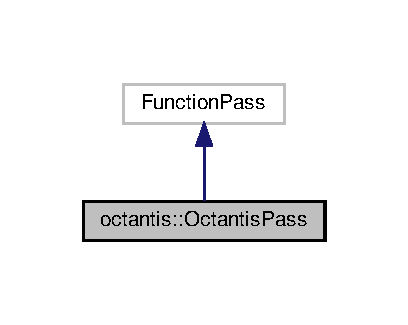
\includegraphics[width=196pt]{structoctantis_1_1OctantisPass__inherit__graph}
\end{center}
\end{figure}


Collaboration diagram for octantis\+:\+:Octantis\+Pass\+:
\nopagebreak
\begin{figure}[H]
\begin{center}
\leavevmode
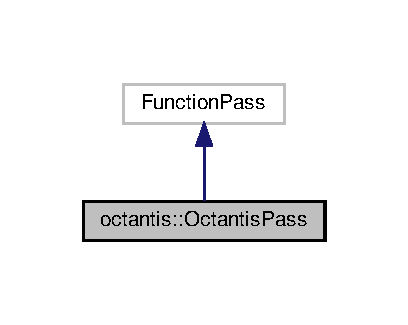
\includegraphics[width=196pt]{structoctantis_1_1OctantisPass__coll__graph}
\end{center}
\end{figure}
\subsection*{Public Member Functions}
\begin{DoxyCompactItemize}
\item 
\hyperlink{structoctantis_1_1OctantisPass_a47caf34ff1187522621d58f636579af7}{Octantis\+Pass} ()
\item 
void \hyperlink{structoctantis_1_1OctantisPass_a9928748c5a25565dec5b98ccba4b12c3}{compile\+And\+Print} ()
\item 
bool \hyperlink{structoctantis_1_1OctantisPass_a2d156c9326f2eaf75969e34aa09df2e5}{run\+On\+Function} (Function \&F) override
\end{DoxyCompactItemize}
\subsection*{Static Public Attributes}
\begin{DoxyCompactItemize}
\item 
static char \hyperlink{structoctantis_1_1OctantisPass_a71e0902b7f244b6aa98ef9f3d34c8637}{ID} = 0
\end{DoxyCompactItemize}


\subsection{Detailed Description}


Definition at line 30 of file Octantis\+Pass.\+cpp.



\subsection{Constructor \& Destructor Documentation}
\mbox{\Hypertarget{structoctantis_1_1OctantisPass_a47caf34ff1187522621d58f636579af7}\label{structoctantis_1_1OctantisPass_a47caf34ff1187522621d58f636579af7}} 
\index{octantis\+::\+Octantis\+Pass@{octantis\+::\+Octantis\+Pass}!Octantis\+Pass@{Octantis\+Pass}}
\index{Octantis\+Pass@{Octantis\+Pass}!octantis\+::\+Octantis\+Pass@{octantis\+::\+Octantis\+Pass}}
\subsubsection{\texorpdfstring{Octantis\+Pass()}{OctantisPass()}}
{\footnotesize\ttfamily octantis\+::\+Octantis\+Pass\+::\+Octantis\+Pass (\begin{DoxyParamCaption}{ }\end{DoxyParamCaption})\hspace{0.3cm}{\ttfamily [inline]}}



Definition at line 32 of file Octantis\+Pass.\+cpp.



\subsection{Member Function Documentation}
\mbox{\Hypertarget{structoctantis_1_1OctantisPass_a9928748c5a25565dec5b98ccba4b12c3}\label{structoctantis_1_1OctantisPass_a9928748c5a25565dec5b98ccba4b12c3}} 
\index{octantis\+::\+Octantis\+Pass@{octantis\+::\+Octantis\+Pass}!compile\+And\+Print@{compile\+And\+Print}}
\index{compile\+And\+Print@{compile\+And\+Print}!octantis\+::\+Octantis\+Pass@{octantis\+::\+Octantis\+Pass}}
\subsubsection{\texorpdfstring{compile\+And\+Print()}{compileAndPrint()}}
{\footnotesize\ttfamily void octantis\+::\+Octantis\+Pass\+::compile\+And\+Print (\begin{DoxyParamCaption}{ }\end{DoxyParamCaption})\hspace{0.3cm}{\ttfamily [inline]}}



Definition at line 34 of file Octantis\+Pass.\+cpp.

\mbox{\Hypertarget{structoctantis_1_1OctantisPass_a2d156c9326f2eaf75969e34aa09df2e5}\label{structoctantis_1_1OctantisPass_a2d156c9326f2eaf75969e34aa09df2e5}} 
\index{octantis\+::\+Octantis\+Pass@{octantis\+::\+Octantis\+Pass}!run\+On\+Function@{run\+On\+Function}}
\index{run\+On\+Function@{run\+On\+Function}!octantis\+::\+Octantis\+Pass@{octantis\+::\+Octantis\+Pass}}
\subsubsection{\texorpdfstring{run\+On\+Function()}{runOnFunction()}}
{\footnotesize\ttfamily bool octantis\+::\+Octantis\+Pass\+::run\+On\+Function (\begin{DoxyParamCaption}\item[{Function \&}]{F }\end{DoxyParamCaption})\hspace{0.3cm}{\ttfamily [inline]}, {\ttfamily [override]}}



Definition at line 40 of file Octantis\+Pass.\+cpp.



\subsection{Member Data Documentation}
\mbox{\Hypertarget{structoctantis_1_1OctantisPass_a71e0902b7f244b6aa98ef9f3d34c8637}\label{structoctantis_1_1OctantisPass_a71e0902b7f244b6aa98ef9f3d34c8637}} 
\index{octantis\+::\+Octantis\+Pass@{octantis\+::\+Octantis\+Pass}!ID@{ID}}
\index{ID@{ID}!octantis\+::\+Octantis\+Pass@{octantis\+::\+Octantis\+Pass}}
\subsubsection{\texorpdfstring{ID}{ID}}
{\footnotesize\ttfamily char Octantis\+Pass\+::\+ID = 0\hspace{0.3cm}{\ttfamily [static]}}



Definition at line 31 of file Octantis\+Pass.\+cpp.



The documentation for this struct was generated from the following file\+:\begin{DoxyCompactItemize}
\item 
/home/andrea/\+Documenti/\+Octantis\+V1.\+0/\+The-\/\+Octantis-\/project/llvm/lib/\+Transforms/\+Octantis/\hyperlink{OctantisPass_8cpp}{Octantis\+Pass.\+cpp}\end{DoxyCompactItemize}

\hypertarget{classoctantis_1_1PrintDexFile}{}\section{octantis\+:\+:Print\+Dex\+File Class Reference}
\label{classoctantis_1_1PrintDexFile}\index{octantis\+::\+Print\+Dex\+File@{octantis\+::\+Print\+Dex\+File}}


Class class useful for the definition of Dexima\textquotesingle{}s configuration file (.dex).  




{\ttfamily \#include $<$Print\+Dex\+File.\+h$>$}

\subsection*{Public Member Functions}
\begin{DoxyCompactItemize}
\item 
\hyperlink{classoctantis_1_1PrintDexFile_a8419b2b9f856dbefc859a563125f203c}{Print\+Dex\+File} (\hyperlink{classoctantis_1_1LiMArray}{Li\+M\+Array} $\ast$comp\+Array, \hyperlink{classoctantis_1_1FiniteStateMachine}{Finite\+State\+Machine} $\ast$comp\+F\+SM, raw\+\_\+ostream $\ast$O\+Stream)
\item 
void \hyperlink{classoctantis_1_1PrintDexFile_a81a7a3c3c35f91aabd83c2902f56dfb1}{print} ()
\begin{DoxyCompactList}\small\item\em It prints the .dex file. \end{DoxyCompactList}\end{DoxyCompactItemize}


\subsection{Detailed Description}
Class class useful for the definition of Dexima\textquotesingle{}s configuration file (.dex). 

\subsection{Constructor \& Destructor Documentation}
\mbox{\Hypertarget{classoctantis_1_1PrintDexFile_a8419b2b9f856dbefc859a563125f203c}\label{classoctantis_1_1PrintDexFile_a8419b2b9f856dbefc859a563125f203c}} 
\index{octantis\+::\+Print\+Dex\+File@{octantis\+::\+Print\+Dex\+File}!Print\+Dex\+File@{Print\+Dex\+File}}
\index{Print\+Dex\+File@{Print\+Dex\+File}!octantis\+::\+Print\+Dex\+File@{octantis\+::\+Print\+Dex\+File}}
\subsubsection{\texorpdfstring{Print\+Dex\+File()}{PrintDexFile()}}
{\footnotesize\ttfamily octantis\+::\+Print\+Dex\+File\+::\+Print\+Dex\+File (\begin{DoxyParamCaption}\item[{\hyperlink{classoctantis_1_1LiMArray}{Li\+M\+Array} $\ast$}]{comp\+Array,  }\item[{\hyperlink{classoctantis_1_1FiniteStateMachine}{Finite\+State\+Machine} $\ast$}]{comp\+F\+SM,  }\item[{raw\+\_\+ostream $\ast$}]{O\+Stream }\end{DoxyParamCaption})\hspace{0.3cm}{\ttfamily [inline]}}



\subsection{Member Function Documentation}
\mbox{\Hypertarget{classoctantis_1_1PrintDexFile_a81a7a3c3c35f91aabd83c2902f56dfb1}\label{classoctantis_1_1PrintDexFile_a81a7a3c3c35f91aabd83c2902f56dfb1}} 
\index{octantis\+::\+Print\+Dex\+File@{octantis\+::\+Print\+Dex\+File}!print@{print}}
\index{print@{print}!octantis\+::\+Print\+Dex\+File@{octantis\+::\+Print\+Dex\+File}}
\subsubsection{\texorpdfstring{print()}{print()}}
{\footnotesize\ttfamily void Print\+Dex\+File\+::print (\begin{DoxyParamCaption}{ }\end{DoxyParamCaption})}



It prints the .dex file. 



The documentation for this class was generated from the following files\+:\begin{DoxyCompactItemize}
\item 
/home/andrea/\+Documenti/\+Octantis\+V1.\+0/\+The-\/\+Octantis-\/project/llvm/lib/\+Transforms/\+Octantis/\hyperlink{PrintDexFile_8h}{Print\+Dex\+File.\+h}\item 
/home/andrea/\+Documenti/\+Octantis\+V1.\+0/\+The-\/\+Octantis-\/project/llvm/lib/\+Transforms/\+Octantis/\hyperlink{PrintDexFile_8cpp}{Print\+Dex\+File.\+cpp}\end{DoxyCompactItemize}

\hypertarget{classoctantis_1_1SchedulingASAP}{}\section{octantis\+:\+:Scheduling\+A\+S\+AP Class Reference}
\label{classoctantis_1_1SchedulingASAP}\index{octantis\+::\+Scheduling\+A\+S\+AP@{octantis\+::\+Scheduling\+A\+S\+AP}}


Class useful for the implementation of the A\+S\+AP Scheduling algorithm.  




{\ttfamily \#include $<$Scheduling\+A\+S\+A\+P.\+h$>$}



Collaboration diagram for octantis\+:\+:Scheduling\+A\+S\+AP\+:
\nopagebreak
\begin{figure}[H]
\begin{center}
\leavevmode
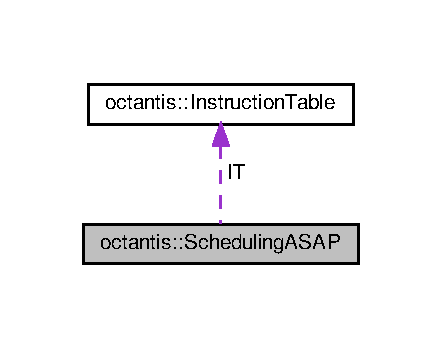
\includegraphics[width=212pt]{classoctantis_1_1SchedulingASAP__coll__graph}
\end{center}
\end{figure}
\subsection*{Public Types}
\begin{DoxyCompactItemize}
\item 
enum \hyperlink{classoctantis_1_1SchedulingASAP_abbd454a56c823d34f835168cc31168f4}{Instr} \{ \newline
\hyperlink{classoctantis_1_1SchedulingASAP_abbd454a56c823d34f835168cc31168f4a1541025cbb5cba48df7df02b247dda94}{alloc}, 
\hyperlink{classoctantis_1_1SchedulingASAP_abbd454a56c823d34f835168cc31168f4a243ac5e1764c17c614cd1593d856ded7}{load}, 
\hyperlink{classoctantis_1_1SchedulingASAP_abbd454a56c823d34f835168cc31168f4a825e4d8f229ce85bc8798614cca89237}{store}, 
\hyperlink{classoctantis_1_1SchedulingASAP_abbd454a56c823d34f835168cc31168f4a71eabbb5cc7e271dc91aadc47e10cf97}{binary}, 
\newline
\hyperlink{classoctantis_1_1SchedulingASAP_abbd454a56c823d34f835168cc31168f4a5972668297576ba95cec790b0628aa7a}{ret}, 
\hyperlink{classoctantis_1_1SchedulingASAP_abbd454a56c823d34f835168cc31168f4afe0f5d927cec721c9936f64edb51ad2f}{ptr}, 
\hyperlink{classoctantis_1_1SchedulingASAP_abbd454a56c823d34f835168cc31168f4a5871b82eb2922df94c8bc366c8ad158f}{unknown}
 \}\begin{DoxyCompactList}\small\item\em Recognized instructions. \end{DoxyCompactList}
\end{DoxyCompactItemize}
\subsection*{Public Member Functions}
\begin{DoxyCompactItemize}
\item 
\hyperlink{classoctantis_1_1SchedulingASAP_a6354db3834d5a1946a9d7fc61f83ac69}{Scheduling\+A\+S\+AP} ()
\begin{DoxyCompactList}\small\item\em Default constructor. \end{DoxyCompactList}\item 
\hyperlink{classoctantis_1_1SchedulingASAP_a8a6fee824cdf5a0a8cde0e98007ff991}{Scheduling\+A\+S\+AP} (Instruction \&I)
\begin{DoxyCompactList}\small\item\em Constructor useful to initialize the Instruction Table. \end{DoxyCompactList}\item 
void \hyperlink{classoctantis_1_1SchedulingASAP_ae901ec5f1113be04c9c28ab0f796c166}{add\+New\+Instruction} (Instruction \&I)
\begin{DoxyCompactList}\small\item\em Function useful to add a new L\+L\+VM IR instruction to the Intruction Table. \end{DoxyCompactList}\item 
void \hyperlink{classoctantis_1_1SchedulingASAP_a8b0a9d978d7b4276b1c741779a5e4191}{increment\+Timer} ()
\begin{DoxyCompactList}\small\item\em Function useful to increment the value of the scheduling timer. \end{DoxyCompactList}\item 
void \hyperlink{classoctantis_1_1SchedulingASAP_a32cbd30ee5e9591898edf498c03ddfaf}{decrement\+Timer} ()
\begin{DoxyCompactList}\small\item\em Function useful to decrement the value of the scheduling timer. \end{DoxyCompactList}\item 
\hyperlink{classoctantis_1_1InstructionTable}{Instruction\+Table} $\ast$ \hyperlink{classoctantis_1_1SchedulingASAP_a2aae2d1a8c0482012ac781faf0a7fd42}{get\+Instruction\+Table} ()
\begin{DoxyCompactList}\small\item\em Function that returns the pointer to the complete Instruction Table. \end{DoxyCompactList}\item 
\hyperlink{classoctantis_1_1SchedulingASAP_abbd454a56c823d34f835168cc31168f4}{Instr} \hyperlink{classoctantis_1_1SchedulingASAP_ac3f43eaa890ea2fe4457d0505b28da77}{identify\+Instr} (Instruction \&I)
\begin{DoxyCompactList}\small\item\em Function that return the type of the instruction passed. \end{DoxyCompactList}\item 
int $\ast$ \hyperlink{classoctantis_1_1SchedulingASAP_a310354a5c7a7613dd66c89b9c358528f}{get\+Real\+Parent} (int $\ast$\&alias\+Parent)
\begin{DoxyCompactList}\small\item\em Function to get the actual source register from which execute the load. \end{DoxyCompactList}\item 
\hyperlink{classoctantis_1_1InstructionTable}{Instruction\+Table} \& \hyperlink{classoctantis_1_1SchedulingASAP_a6c61709d8b29672b8e6cad471b81808d}{get\+IT} ()
\begin{DoxyCompactList}\small\item\em Function to return the pointer to the Instruction Table. \end{DoxyCompactList}\item 
void \hyperlink{classoctantis_1_1SchedulingASAP_ae3df036361ff37d74ca915487f1be0b4}{print\+Alias\+Map} ()
\end{DoxyCompactItemize}
\subsection*{Public Attributes}
\begin{DoxyCompactItemize}
\item 
\hyperlink{classoctantis_1_1InstructionTable}{Instruction\+Table} \hyperlink{classoctantis_1_1SchedulingASAP_ac53b361e1b4663c158238d93b931dce3}{IT}
\end{DoxyCompactItemize}


\subsection{Detailed Description}
Class useful for the implementation of the A\+S\+AP Scheduling algorithm. 

Definition at line 28 of file Scheduling\+A\+S\+A\+P.\+h.



\subsection{Member Enumeration Documentation}
\mbox{\Hypertarget{classoctantis_1_1SchedulingASAP_abbd454a56c823d34f835168cc31168f4}\label{classoctantis_1_1SchedulingASAP_abbd454a56c823d34f835168cc31168f4}} 
\index{octantis\+::\+Scheduling\+A\+S\+AP@{octantis\+::\+Scheduling\+A\+S\+AP}!Instr@{Instr}}
\index{Instr@{Instr}!octantis\+::\+Scheduling\+A\+S\+AP@{octantis\+::\+Scheduling\+A\+S\+AP}}
\subsubsection{\texorpdfstring{Instr}{Instr}}
{\footnotesize\ttfamily enum \hyperlink{classoctantis_1_1SchedulingASAP_abbd454a56c823d34f835168cc31168f4}{octantis\+::\+Scheduling\+A\+S\+A\+P\+::\+Instr}}



Recognized instructions. 

\begin{DoxyEnumFields}{Enumerator}
\raisebox{\heightof{T}}[0pt][0pt]{\index{alloc@{alloc}!octantis\+::\+Scheduling\+A\+S\+AP@{octantis\+::\+Scheduling\+A\+S\+AP}}\index{octantis\+::\+Scheduling\+A\+S\+AP@{octantis\+::\+Scheduling\+A\+S\+AP}!alloc@{alloc}}}\mbox{\Hypertarget{classoctantis_1_1SchedulingASAP_abbd454a56c823d34f835168cc31168f4a1541025cbb5cba48df7df02b247dda94}\label{classoctantis_1_1SchedulingASAP_abbd454a56c823d34f835168cc31168f4a1541025cbb5cba48df7df02b247dda94}} 
alloc&\\
\hline

\raisebox{\heightof{T}}[0pt][0pt]{\index{load@{load}!octantis\+::\+Scheduling\+A\+S\+AP@{octantis\+::\+Scheduling\+A\+S\+AP}}\index{octantis\+::\+Scheduling\+A\+S\+AP@{octantis\+::\+Scheduling\+A\+S\+AP}!load@{load}}}\mbox{\Hypertarget{classoctantis_1_1SchedulingASAP_abbd454a56c823d34f835168cc31168f4a243ac5e1764c17c614cd1593d856ded7}\label{classoctantis_1_1SchedulingASAP_abbd454a56c823d34f835168cc31168f4a243ac5e1764c17c614cd1593d856ded7}} 
load&\\
\hline

\raisebox{\heightof{T}}[0pt][0pt]{\index{store@{store}!octantis\+::\+Scheduling\+A\+S\+AP@{octantis\+::\+Scheduling\+A\+S\+AP}}\index{octantis\+::\+Scheduling\+A\+S\+AP@{octantis\+::\+Scheduling\+A\+S\+AP}!store@{store}}}\mbox{\Hypertarget{classoctantis_1_1SchedulingASAP_abbd454a56c823d34f835168cc31168f4a825e4d8f229ce85bc8798614cca89237}\label{classoctantis_1_1SchedulingASAP_abbd454a56c823d34f835168cc31168f4a825e4d8f229ce85bc8798614cca89237}} 
store&\\
\hline

\raisebox{\heightof{T}}[0pt][0pt]{\index{binary@{binary}!octantis\+::\+Scheduling\+A\+S\+AP@{octantis\+::\+Scheduling\+A\+S\+AP}}\index{octantis\+::\+Scheduling\+A\+S\+AP@{octantis\+::\+Scheduling\+A\+S\+AP}!binary@{binary}}}\mbox{\Hypertarget{classoctantis_1_1SchedulingASAP_abbd454a56c823d34f835168cc31168f4a71eabbb5cc7e271dc91aadc47e10cf97}\label{classoctantis_1_1SchedulingASAP_abbd454a56c823d34f835168cc31168f4a71eabbb5cc7e271dc91aadc47e10cf97}} 
binary&\\
\hline

\raisebox{\heightof{T}}[0pt][0pt]{\index{ret@{ret}!octantis\+::\+Scheduling\+A\+S\+AP@{octantis\+::\+Scheduling\+A\+S\+AP}}\index{octantis\+::\+Scheduling\+A\+S\+AP@{octantis\+::\+Scheduling\+A\+S\+AP}!ret@{ret}}}\mbox{\Hypertarget{classoctantis_1_1SchedulingASAP_abbd454a56c823d34f835168cc31168f4a5972668297576ba95cec790b0628aa7a}\label{classoctantis_1_1SchedulingASAP_abbd454a56c823d34f835168cc31168f4a5972668297576ba95cec790b0628aa7a}} 
ret&\\
\hline

\raisebox{\heightof{T}}[0pt][0pt]{\index{ptr@{ptr}!octantis\+::\+Scheduling\+A\+S\+AP@{octantis\+::\+Scheduling\+A\+S\+AP}}\index{octantis\+::\+Scheduling\+A\+S\+AP@{octantis\+::\+Scheduling\+A\+S\+AP}!ptr@{ptr}}}\mbox{\Hypertarget{classoctantis_1_1SchedulingASAP_abbd454a56c823d34f835168cc31168f4afe0f5d927cec721c9936f64edb51ad2f}\label{classoctantis_1_1SchedulingASAP_abbd454a56c823d34f835168cc31168f4afe0f5d927cec721c9936f64edb51ad2f}} 
ptr&\\
\hline

\raisebox{\heightof{T}}[0pt][0pt]{\index{unknown@{unknown}!octantis\+::\+Scheduling\+A\+S\+AP@{octantis\+::\+Scheduling\+A\+S\+AP}}\index{octantis\+::\+Scheduling\+A\+S\+AP@{octantis\+::\+Scheduling\+A\+S\+AP}!unknown@{unknown}}}\mbox{\Hypertarget{classoctantis_1_1SchedulingASAP_abbd454a56c823d34f835168cc31168f4a5871b82eb2922df94c8bc366c8ad158f}\label{classoctantis_1_1SchedulingASAP_abbd454a56c823d34f835168cc31168f4a5871b82eb2922df94c8bc366c8ad158f}} 
unknown&\\
\hline

\end{DoxyEnumFields}


Definition at line 32 of file Scheduling\+A\+S\+A\+P.\+h.



\subsection{Constructor \& Destructor Documentation}
\mbox{\Hypertarget{classoctantis_1_1SchedulingASAP_a6354db3834d5a1946a9d7fc61f83ac69}\label{classoctantis_1_1SchedulingASAP_a6354db3834d5a1946a9d7fc61f83ac69}} 
\index{octantis\+::\+Scheduling\+A\+S\+AP@{octantis\+::\+Scheduling\+A\+S\+AP}!Scheduling\+A\+S\+AP@{Scheduling\+A\+S\+AP}}
\index{Scheduling\+A\+S\+AP@{Scheduling\+A\+S\+AP}!octantis\+::\+Scheduling\+A\+S\+AP@{octantis\+::\+Scheduling\+A\+S\+AP}}
\subsubsection{\texorpdfstring{Scheduling\+A\+S\+A\+P()}{SchedulingASAP()}\hspace{0.1cm}{\footnotesize\ttfamily [1/2]}}
{\footnotesize\ttfamily Scheduling\+A\+S\+A\+P\+::\+Scheduling\+A\+S\+AP (\begin{DoxyParamCaption}{ }\end{DoxyParamCaption})}



Default constructor. 



Definition at line 29 of file Scheduling\+A\+S\+A\+P.\+cpp.

\mbox{\Hypertarget{classoctantis_1_1SchedulingASAP_a8a6fee824cdf5a0a8cde0e98007ff991}\label{classoctantis_1_1SchedulingASAP_a8a6fee824cdf5a0a8cde0e98007ff991}} 
\index{octantis\+::\+Scheduling\+A\+S\+AP@{octantis\+::\+Scheduling\+A\+S\+AP}!Scheduling\+A\+S\+AP@{Scheduling\+A\+S\+AP}}
\index{Scheduling\+A\+S\+AP@{Scheduling\+A\+S\+AP}!octantis\+::\+Scheduling\+A\+S\+AP@{octantis\+::\+Scheduling\+A\+S\+AP}}
\subsubsection{\texorpdfstring{Scheduling\+A\+S\+A\+P()}{SchedulingASAP()}\hspace{0.1cm}{\footnotesize\ttfamily [2/2]}}
{\footnotesize\ttfamily Scheduling\+A\+S\+A\+P\+::\+Scheduling\+A\+S\+AP (\begin{DoxyParamCaption}\item[{Instruction \&}]{I }\end{DoxyParamCaption})}



Constructor useful to initialize the Instruction Table. 



Definition at line 35 of file Scheduling\+A\+S\+A\+P.\+cpp.



\subsection{Member Function Documentation}
\mbox{\Hypertarget{classoctantis_1_1SchedulingASAP_ae901ec5f1113be04c9c28ab0f796c166}\label{classoctantis_1_1SchedulingASAP_ae901ec5f1113be04c9c28ab0f796c166}} 
\index{octantis\+::\+Scheduling\+A\+S\+AP@{octantis\+::\+Scheduling\+A\+S\+AP}!add\+New\+Instruction@{add\+New\+Instruction}}
\index{add\+New\+Instruction@{add\+New\+Instruction}!octantis\+::\+Scheduling\+A\+S\+AP@{octantis\+::\+Scheduling\+A\+S\+AP}}
\subsubsection{\texorpdfstring{add\+New\+Instruction()}{addNewInstruction()}}
{\footnotesize\ttfamily void Scheduling\+A\+S\+A\+P\+::add\+New\+Instruction (\begin{DoxyParamCaption}\item[{Instruction \&}]{I }\end{DoxyParamCaption})}



Function useful to add a new L\+L\+VM IR instruction to the Intruction Table. 



Definition at line 41 of file Scheduling\+A\+S\+A\+P.\+cpp.

\mbox{\Hypertarget{classoctantis_1_1SchedulingASAP_a32cbd30ee5e9591898edf498c03ddfaf}\label{classoctantis_1_1SchedulingASAP_a32cbd30ee5e9591898edf498c03ddfaf}} 
\index{octantis\+::\+Scheduling\+A\+S\+AP@{octantis\+::\+Scheduling\+A\+S\+AP}!decrement\+Timer@{decrement\+Timer}}
\index{decrement\+Timer@{decrement\+Timer}!octantis\+::\+Scheduling\+A\+S\+AP@{octantis\+::\+Scheduling\+A\+S\+AP}}
\subsubsection{\texorpdfstring{decrement\+Timer()}{decrementTimer()}}
{\footnotesize\ttfamily void Scheduling\+A\+S\+A\+P\+::decrement\+Timer (\begin{DoxyParamCaption}{ }\end{DoxyParamCaption})}



Function useful to decrement the value of the scheduling timer. 



Definition at line 218 of file Scheduling\+A\+S\+A\+P.\+cpp.

\mbox{\Hypertarget{classoctantis_1_1SchedulingASAP_a2aae2d1a8c0482012ac781faf0a7fd42}\label{classoctantis_1_1SchedulingASAP_a2aae2d1a8c0482012ac781faf0a7fd42}} 
\index{octantis\+::\+Scheduling\+A\+S\+AP@{octantis\+::\+Scheduling\+A\+S\+AP}!get\+Instruction\+Table@{get\+Instruction\+Table}}
\index{get\+Instruction\+Table@{get\+Instruction\+Table}!octantis\+::\+Scheduling\+A\+S\+AP@{octantis\+::\+Scheduling\+A\+S\+AP}}
\subsubsection{\texorpdfstring{get\+Instruction\+Table()}{getInstructionTable()}}
{\footnotesize\ttfamily \hyperlink{classoctantis_1_1InstructionTable}{Instruction\+Table} $\ast$ Scheduling\+A\+S\+A\+P\+::get\+Instruction\+Table (\begin{DoxyParamCaption}{ }\end{DoxyParamCaption})}



Function that returns the pointer to the complete Instruction Table. 



Definition at line 224 of file Scheduling\+A\+S\+A\+P.\+cpp.

\mbox{\Hypertarget{classoctantis_1_1SchedulingASAP_a6c61709d8b29672b8e6cad471b81808d}\label{classoctantis_1_1SchedulingASAP_a6c61709d8b29672b8e6cad471b81808d}} 
\index{octantis\+::\+Scheduling\+A\+S\+AP@{octantis\+::\+Scheduling\+A\+S\+AP}!get\+IT@{get\+IT}}
\index{get\+IT@{get\+IT}!octantis\+::\+Scheduling\+A\+S\+AP@{octantis\+::\+Scheduling\+A\+S\+AP}}
\subsubsection{\texorpdfstring{get\+I\+T()}{getIT()}}
{\footnotesize\ttfamily \hyperlink{classoctantis_1_1InstructionTable}{Instruction\+Table} \& Scheduling\+A\+S\+A\+P\+::get\+IT (\begin{DoxyParamCaption}{ }\end{DoxyParamCaption})}



Function to return the pointer to the Instruction Table. 



Definition at line 313 of file Scheduling\+A\+S\+A\+P.\+cpp.

\mbox{\Hypertarget{classoctantis_1_1SchedulingASAP_a310354a5c7a7613dd66c89b9c358528f}\label{classoctantis_1_1SchedulingASAP_a310354a5c7a7613dd66c89b9c358528f}} 
\index{octantis\+::\+Scheduling\+A\+S\+AP@{octantis\+::\+Scheduling\+A\+S\+AP}!get\+Real\+Parent@{get\+Real\+Parent}}
\index{get\+Real\+Parent@{get\+Real\+Parent}!octantis\+::\+Scheduling\+A\+S\+AP@{octantis\+::\+Scheduling\+A\+S\+AP}}
\subsubsection{\texorpdfstring{get\+Real\+Parent()}{getRealParent()}}
{\footnotesize\ttfamily int $\ast$ Scheduling\+A\+S\+A\+P\+::get\+Real\+Parent (\begin{DoxyParamCaption}\item[{int $\ast$\&}]{alias\+Parent }\end{DoxyParamCaption})}



Function to get the actual source register from which execute the load. 



Definition at line 299 of file Scheduling\+A\+S\+A\+P.\+cpp.

\mbox{\Hypertarget{classoctantis_1_1SchedulingASAP_ac3f43eaa890ea2fe4457d0505b28da77}\label{classoctantis_1_1SchedulingASAP_ac3f43eaa890ea2fe4457d0505b28da77}} 
\index{octantis\+::\+Scheduling\+A\+S\+AP@{octantis\+::\+Scheduling\+A\+S\+AP}!identify\+Instr@{identify\+Instr}}
\index{identify\+Instr@{identify\+Instr}!octantis\+::\+Scheduling\+A\+S\+AP@{octantis\+::\+Scheduling\+A\+S\+AP}}
\subsubsection{\texorpdfstring{identify\+Instr()}{identifyInstr()}}
{\footnotesize\ttfamily \hyperlink{classoctantis_1_1SchedulingASAP_abbd454a56c823d34f835168cc31168f4}{Scheduling\+A\+S\+A\+P\+::\+Instr} Scheduling\+A\+S\+A\+P\+::identify\+Instr (\begin{DoxyParamCaption}\item[{Instruction \&}]{I }\end{DoxyParamCaption})}



Function that return the type of the instruction passed. 



Definition at line 230 of file Scheduling\+A\+S\+A\+P.\+cpp.

\mbox{\Hypertarget{classoctantis_1_1SchedulingASAP_a8b0a9d978d7b4276b1c741779a5e4191}\label{classoctantis_1_1SchedulingASAP_a8b0a9d978d7b4276b1c741779a5e4191}} 
\index{octantis\+::\+Scheduling\+A\+S\+AP@{octantis\+::\+Scheduling\+A\+S\+AP}!increment\+Timer@{increment\+Timer}}
\index{increment\+Timer@{increment\+Timer}!octantis\+::\+Scheduling\+A\+S\+AP@{octantis\+::\+Scheduling\+A\+S\+AP}}
\subsubsection{\texorpdfstring{increment\+Timer()}{incrementTimer()}}
{\footnotesize\ttfamily void Scheduling\+A\+S\+A\+P\+::increment\+Timer (\begin{DoxyParamCaption}{ }\end{DoxyParamCaption})}



Function useful to increment the value of the scheduling timer. 



Definition at line 212 of file Scheduling\+A\+S\+A\+P.\+cpp.

\mbox{\Hypertarget{classoctantis_1_1SchedulingASAP_ae3df036361ff37d74ca915487f1be0b4}\label{classoctantis_1_1SchedulingASAP_ae3df036361ff37d74ca915487f1be0b4}} 
\index{octantis\+::\+Scheduling\+A\+S\+AP@{octantis\+::\+Scheduling\+A\+S\+AP}!print\+Alias\+Map@{print\+Alias\+Map}}
\index{print\+Alias\+Map@{print\+Alias\+Map}!octantis\+::\+Scheduling\+A\+S\+AP@{octantis\+::\+Scheduling\+A\+S\+AP}}
\subsubsection{\texorpdfstring{print\+Alias\+Map()}{printAliasMap()}}
{\footnotesize\ttfamily void Scheduling\+A\+S\+A\+P\+::print\+Alias\+Map (\begin{DoxyParamCaption}{ }\end{DoxyParamCaption})}



Definition at line 321 of file Scheduling\+A\+S\+A\+P.\+cpp.



\subsection{Member Data Documentation}
\mbox{\Hypertarget{classoctantis_1_1SchedulingASAP_ac53b361e1b4663c158238d93b931dce3}\label{classoctantis_1_1SchedulingASAP_ac53b361e1b4663c158238d93b931dce3}} 
\index{octantis\+::\+Scheduling\+A\+S\+AP@{octantis\+::\+Scheduling\+A\+S\+AP}!IT@{IT}}
\index{IT@{IT}!octantis\+::\+Scheduling\+A\+S\+AP@{octantis\+::\+Scheduling\+A\+S\+AP}}
\subsubsection{\texorpdfstring{IT}{IT}}
{\footnotesize\ttfamily \hyperlink{classoctantis_1_1InstructionTable}{Instruction\+Table} octantis\+::\+Scheduling\+A\+S\+A\+P\+::\+IT}



Definition at line 101 of file Scheduling\+A\+S\+A\+P.\+h.



The documentation for this class was generated from the following files\+:\begin{DoxyCompactItemize}
\item 
/home/andrea/\+Documenti/\+Octantis\+V1.\+0/\+The-\/\+Octantis-\/project/llvm/lib/\+Transforms/\+Octantis/\hyperlink{SchedulingASAP_8h}{Scheduling\+A\+S\+A\+P.\+h}\item 
/home/andrea/\+Documenti/\+Octantis\+V1.\+0/\+The-\/\+Octantis-\/project/llvm/lib/\+Transforms/\+Octantis/\hyperlink{SchedulingASAP_8cpp}{Scheduling\+A\+S\+A\+P.\+cpp}\end{DoxyCompactItemize}

\chapter{File Documentation}
\hypertarget{README_8md}{}\section{R\+E\+A\+D\+M\+E.\+md File Reference}
\label{README_8md}\index{R\+E\+A\+D\+M\+E.\+md@{R\+E\+A\+D\+M\+E.\+md}}

\hypertarget{AdditionalLogicPorts_8cpp}{}\section{/home/andrea/\+Documenti/\+Octantis\+V1.0/\+The-\/\+Octantis-\/project/llvm/lib/\+Transforms/\+Octantis/\+Additional\+Logic\+Ports.cpp File Reference}
\label{AdditionalLogicPorts_8cpp}\index{/home/andrea/\+Documenti/\+Octantis\+V1.\+0/\+The-\/\+Octantis-\/project/llvm/lib/\+Transforms/\+Octantis/\+Additional\+Logic\+Ports.\+cpp@{/home/andrea/\+Documenti/\+Octantis\+V1.\+0/\+The-\/\+Octantis-\/project/llvm/lib/\+Transforms/\+Octantis/\+Additional\+Logic\+Ports.\+cpp}}
{\ttfamily \#include \char`\"{}Additional\+Logic\+Ports.\+h\char`\"{}}\newline
{\ttfamily \#include \char`\"{}llvm/\+Support/raw\+\_\+ostream.\+h\char`\"{}}\newline
Include dependency graph for Additional\+Logic\+Ports.\+cpp\+:
\nopagebreak
\begin{figure}[H]
\begin{center}
\leavevmode
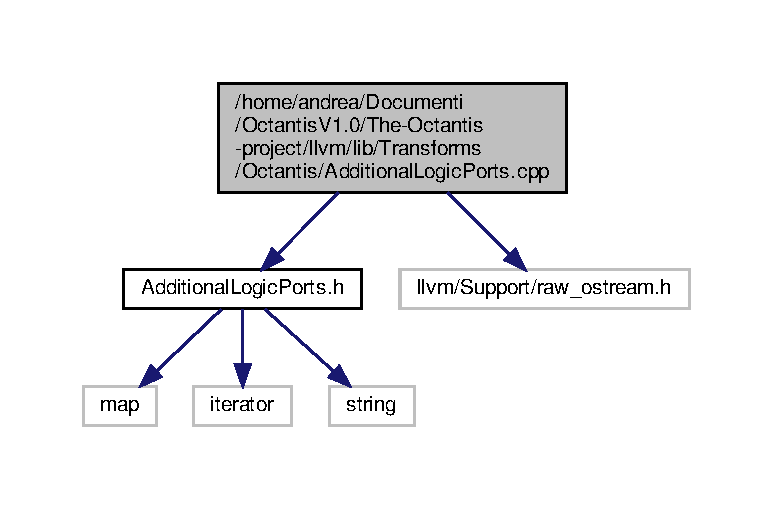
\includegraphics[width=350pt]{AdditionalLogicPorts_8cpp__incl}
\end{center}
\end{figure}

\hypertarget{AdditionalLogicPorts_8h}{}\section{/home/andrea/\+Documenti/\+Octantis\+V1.0/\+The-\/\+Octantis-\/project/llvm/lib/\+Transforms/\+Octantis/\+Additional\+Logic\+Ports.h File Reference}
\label{AdditionalLogicPorts_8h}\index{/home/andrea/\+Documenti/\+Octantis\+V1.\+0/\+The-\/\+Octantis-\/project/llvm/lib/\+Transforms/\+Octantis/\+Additional\+Logic\+Ports.\+h@{/home/andrea/\+Documenti/\+Octantis\+V1.\+0/\+The-\/\+Octantis-\/project/llvm/lib/\+Transforms/\+Octantis/\+Additional\+Logic\+Ports.\+h}}
{\ttfamily \#include $<$map$>$}\newline
{\ttfamily \#include $<$iterator$>$}\newline
{\ttfamily \#include $<$string$>$}\newline
Include dependency graph for Additional\+Logic\+Ports.\+h\+:
\nopagebreak
\begin{figure}[H]
\begin{center}
\leavevmode
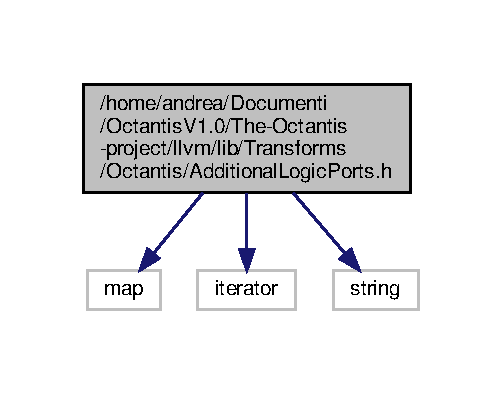
\includegraphics[width=241pt]{AdditionalLogicPorts_8h__incl}
\end{center}
\end{figure}
This graph shows which files directly or indirectly include this file\+:
\nopagebreak
\begin{figure}[H]
\begin{center}
\leavevmode
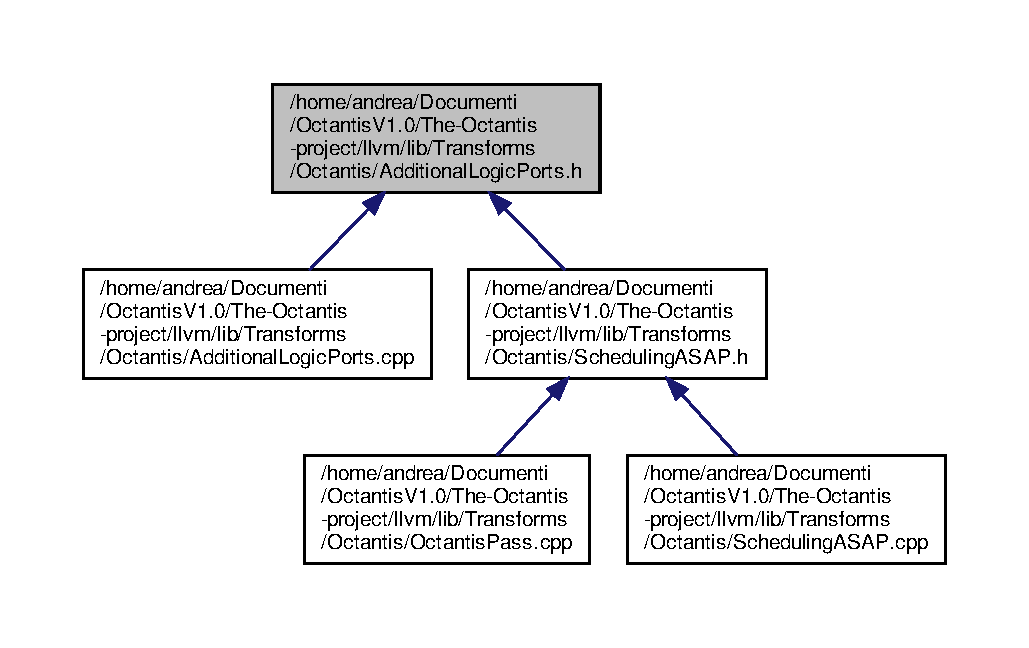
\includegraphics[width=350pt]{AdditionalLogicPorts_8h__dep__incl}
\end{center}
\end{figure}
\subsection*{Classes}
\begin{DoxyCompactItemize}
\item 
class \hyperlink{classoctantis_1_1AdditionalLogicPorts}{octantis\+::\+Additional\+Logic\+Ports}
\end{DoxyCompactItemize}
\subsection*{Namespaces}
\begin{DoxyCompactItemize}
\item 
 \hyperlink{namespaceoctantis}{octantis}
\end{DoxyCompactItemize}

\hypertarget{FiniteStateMachine_8cpp}{}\section{/home/andrea/\+Documenti/\+Octantis\+V1.0/\+The-\/\+Octantis-\/project/llvm/lib/\+Transforms/\+Octantis/\+Finite\+State\+Machine.cpp File Reference}
\label{FiniteStateMachine_8cpp}\index{/home/andrea/\+Documenti/\+Octantis\+V1.\+0/\+The-\/\+Octantis-\/project/llvm/lib/\+Transforms/\+Octantis/\+Finite\+State\+Machine.\+cpp@{/home/andrea/\+Documenti/\+Octantis\+V1.\+0/\+The-\/\+Octantis-\/project/llvm/lib/\+Transforms/\+Octantis/\+Finite\+State\+Machine.\+cpp}}
{\ttfamily \#include \char`\"{}Finite\+State\+Machine.\+h\char`\"{}}\newline
{\ttfamily \#include \char`\"{}llvm/\+Support/raw\+\_\+ostream.\+h\char`\"{}}\newline
Include dependency graph for Finite\+State\+Machine.\+cpp\+:

\hypertarget{FiniteStateMachine_8h}{}\section{/home/andrea/\+Documenti/\+Octantis\+V1.0/\+The-\/\+Octantis-\/project/llvm/lib/\+Transforms/\+Octantis/\+Finite\+State\+Machine.h File Reference}
\label{FiniteStateMachine_8h}\index{/home/andrea/\+Documenti/\+Octantis\+V1.\+0/\+The-\/\+Octantis-\/project/llvm/lib/\+Transforms/\+Octantis/\+Finite\+State\+Machine.\+h@{/home/andrea/\+Documenti/\+Octantis\+V1.\+0/\+The-\/\+Octantis-\/project/llvm/lib/\+Transforms/\+Octantis/\+Finite\+State\+Machine.\+h}}
{\ttfamily \#include $<$map$>$}\newline
{\ttfamily \#include $<$list$>$}\newline
{\ttfamily \#include $<$iterator$>$}\newline
Include dependency graph for Finite\+State\+Machine.\+h\+:
\nopagebreak
\begin{figure}[H]
\begin{center}
\leavevmode
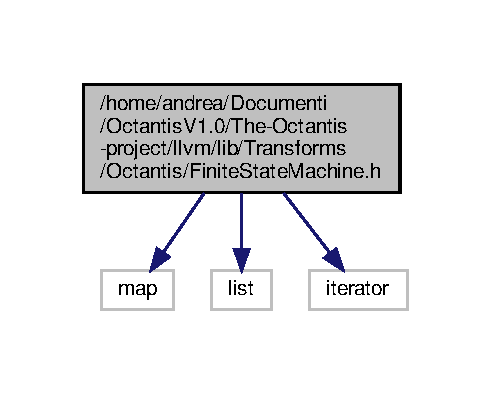
\includegraphics[width=236pt]{FiniteStateMachine_8h__incl}
\end{center}
\end{figure}
This graph shows which files directly or indirectly include this file\+:
\nopagebreak
\begin{figure}[H]
\begin{center}
\leavevmode
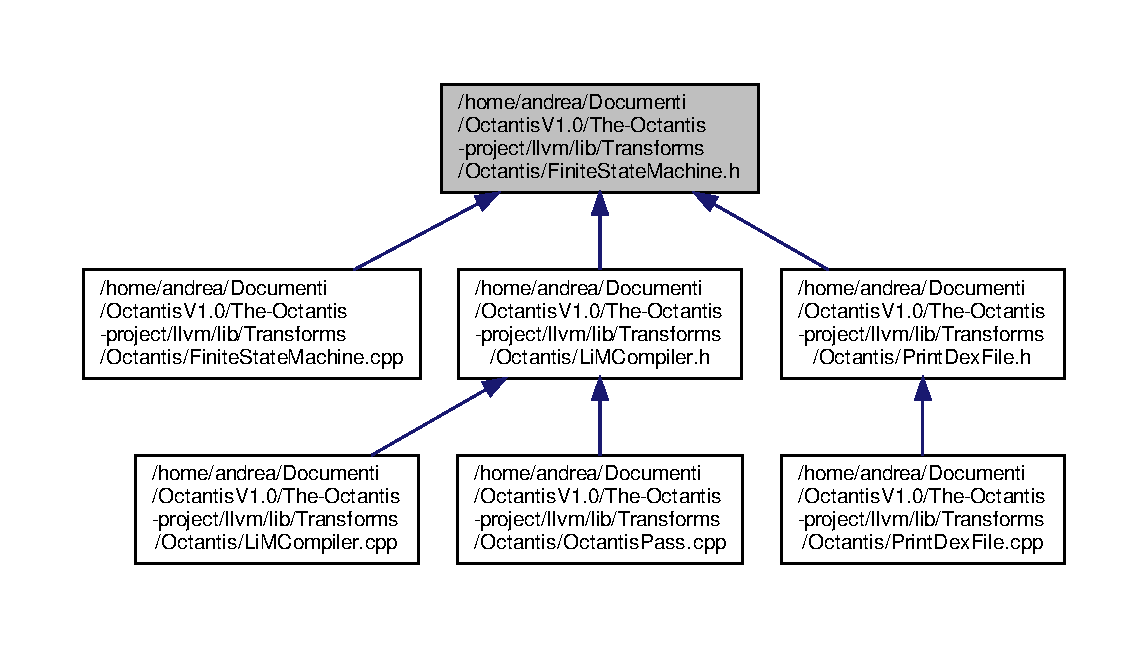
\includegraphics[width=350pt]{FiniteStateMachine_8h__dep__incl}
\end{center}
\end{figure}
\subsection*{Classes}
\begin{DoxyCompactItemize}
\item 
class \hyperlink{classoctantis_1_1FiniteStateMachine}{octantis\+::\+Finite\+State\+Machine}
\begin{DoxyCompactList}\small\item\em Class useful for the definition of the F\+SM of the algorithm. \end{DoxyCompactList}\end{DoxyCompactItemize}
\subsection*{Namespaces}
\begin{DoxyCompactItemize}
\item 
 \hyperlink{namespaceoctantis}{octantis}
\end{DoxyCompactItemize}

\hypertarget{InstructionTable_8cpp}{}\section{/home/andrea/\+Documenti/\+Octantis\+V1.0/\+The-\/\+Octantis-\/project/llvm/lib/\+Transforms/\+Octantis/\+Instruction\+Table.cpp File Reference}
\label{InstructionTable_8cpp}\index{/home/andrea/\+Documenti/\+Octantis\+V1.\+0/\+The-\/\+Octantis-\/project/llvm/lib/\+Transforms/\+Octantis/\+Instruction\+Table.\+cpp@{/home/andrea/\+Documenti/\+Octantis\+V1.\+0/\+The-\/\+Octantis-\/project/llvm/lib/\+Transforms/\+Octantis/\+Instruction\+Table.\+cpp}}
{\ttfamily \#include \char`\"{}Instruction\+Table.\+h\char`\"{}}\newline
{\ttfamily \#include $<$algorithm$>$}\newline
Include dependency graph for Instruction\+Table.\+cpp\+:
\nopagebreak
\begin{figure}[H]
\begin{center}
\leavevmode
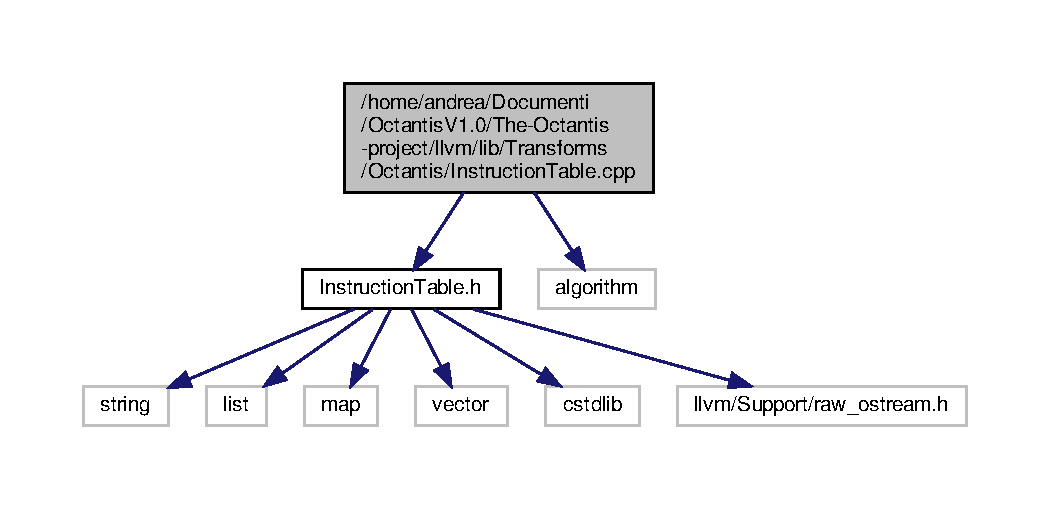
\includegraphics[width=350pt]{InstructionTable_8cpp__incl}
\end{center}
\end{figure}

\hypertarget{InstructionTable_8h}{}\section{/home/andrea/\+Documenti/\+Octantis\+V1.0/\+The-\/\+Octantis-\/project/llvm/lib/\+Transforms/\+Octantis/\+Instruction\+Table.h File Reference}
\label{InstructionTable_8h}\index{/home/andrea/\+Documenti/\+Octantis\+V1.\+0/\+The-\/\+Octantis-\/project/llvm/lib/\+Transforms/\+Octantis/\+Instruction\+Table.\+h@{/home/andrea/\+Documenti/\+Octantis\+V1.\+0/\+The-\/\+Octantis-\/project/llvm/lib/\+Transforms/\+Octantis/\+Instruction\+Table.\+h}}
{\ttfamily \#include $<$string$>$}\newline
{\ttfamily \#include $<$list$>$}\newline
{\ttfamily \#include $<$map$>$}\newline
{\ttfamily \#include $<$cstdlib$>$}\newline
{\ttfamily \#include \char`\"{}llvm/\+Support/raw\+\_\+ostream.\+h\char`\"{}}\newline
Include dependency graph for Instruction\+Table.\+h\+:
% FIG 0
This graph shows which files directly or indirectly include this file\+:
% FIG 1
\subsection*{Classes}
\begin{DoxyCompactItemize}
\item 
class \hyperlink{classoctantis_1_1InstructionTable}{octantis\+::\+Instruction\+Table}
\begin{DoxyCompactList}\small\item\em Class useful to store the instructions that will be scheduled on the LiM architecture. \end{DoxyCompactList}\item 
struct \hyperlink{structoctantis_1_1InstructionTable_1_1instructionData}{octantis\+::\+Instruction\+Table\+::instruction\+Data}
\begin{DoxyCompactList}\small\item\em Structure useful to store the information related to each L\+L\+VM instruction. \end{DoxyCompactList}\item 
struct \hyperlink{structoctantis_1_1InstructionTable_1_1allocatedData}{octantis\+::\+Instruction\+Table\+::allocated\+Data}
\end{DoxyCompactItemize}
\subsection*{Namespaces}
\begin{DoxyCompactItemize}
\item 
 \hyperlink{namespaceoctantis}{octantis}
\end{DoxyCompactItemize}

\hypertarget{LiMArray_8cpp}{}\section{/home/andrea/\+Documenti/\+Octantis\+V1.0/\+The-\/\+Octantis-\/project/llvm/lib/\+Transforms/\+Octantis/\+Li\+M\+Array.cpp File Reference}
\label{LiMArray_8cpp}\index{/home/andrea/\+Documenti/\+Octantis\+V1.\+0/\+The-\/\+Octantis-\/project/llvm/lib/\+Transforms/\+Octantis/\+Li\+M\+Array.\+cpp@{/home/andrea/\+Documenti/\+Octantis\+V1.\+0/\+The-\/\+Octantis-\/project/llvm/lib/\+Transforms/\+Octantis/\+Li\+M\+Array.\+cpp}}
{\ttfamily \#include \char`\"{}Li\+M\+Array.\+h\char`\"{}}\newline
{\ttfamily \#include \char`\"{}Operations\+Implemented.\+h\char`\"{}}\newline
{\ttfamily \#include \char`\"{}llvm/\+Support/raw\+\_\+ostream.\+h\char`\"{}}\newline
Include dependency graph for Li\+M\+Array.\+cpp\+:
% FIG 0

\hypertarget{LiMArray_8h}{}\section{/home/andrea/\+Documenti/\+Octantis\+V1.0/\+The-\/\+Octantis-\/project/llvm/lib/\+Transforms/\+Octantis/\+Li\+M\+Array.h File Reference}
\label{LiMArray_8h}\index{/home/andrea/\+Documenti/\+Octantis\+V1.\+0/\+The-\/\+Octantis-\/project/llvm/lib/\+Transforms/\+Octantis/\+Li\+M\+Array.\+h@{/home/andrea/\+Documenti/\+Octantis\+V1.\+0/\+The-\/\+Octantis-\/project/llvm/lib/\+Transforms/\+Octantis/\+Li\+M\+Array.\+h}}
{\ttfamily \#include $<$map$>$}\newline
{\ttfamily \#include $<$list$>$}\newline
{\ttfamily \#include $<$iterator$>$}\newline
{\ttfamily \#include $<$string$>$}\newline
Include dependency graph for Li\+M\+Array.\+h\+:
% FIG 0
This graph shows which files directly or indirectly include this file\+:
% FIG 1
\subsection*{Classes}
\begin{DoxyCompactItemize}
\item 
class \hyperlink{classoctantis_1_1LiMArray}{octantis\+::\+Li\+M\+Array}
\begin{DoxyCompactList}\small\item\em Class implementing the necessary structures to model the LiM Unit. \end{DoxyCompactList}\item 
struct \hyperlink{structoctantis_1_1LiMArray_1_1LiMRow}{octantis\+::\+Li\+M\+Array\+::\+Li\+M\+Row}
\begin{DoxyCompactList}\small\item\em Lim row description. \end{DoxyCompactList}\end{DoxyCompactItemize}
\subsection*{Namespaces}
\begin{DoxyCompactItemize}
\item 
 \hyperlink{namespaceoctantis}{octantis}
\end{DoxyCompactItemize}

\hypertarget{LiMCompiler_8cpp}{}\section{/home/andrea/\+Documenti/\+Octantis\+V1.0/\+The-\/\+Octantis-\/project/llvm/lib/\+Transforms/\+Octantis/\+Li\+M\+Compiler.cpp File Reference}
\label{LiMCompiler_8cpp}\index{/home/andrea/\+Documenti/\+Octantis\+V1.\+0/\+The-\/\+Octantis-\/project/llvm/lib/\+Transforms/\+Octantis/\+Li\+M\+Compiler.\+cpp@{/home/andrea/\+Documenti/\+Octantis\+V1.\+0/\+The-\/\+Octantis-\/project/llvm/lib/\+Transforms/\+Octantis/\+Li\+M\+Compiler.\+cpp}}
{\ttfamily \#include $<$string$>$}\newline
{\ttfamily \#include \char`\"{}Li\+M\+Compiler.\+h\char`\"{}}\newline
{\ttfamily \#include \char`\"{}Li\+M\+Array.\+h\char`\"{}}\newline
{\ttfamily \#include \char`\"{}Operations\+Implemented.\+h\char`\"{}}\newline
Include dependency graph for Li\+M\+Compiler.\+cpp\+:
\nopagebreak
\begin{figure}[H]
\begin{center}
\leavevmode
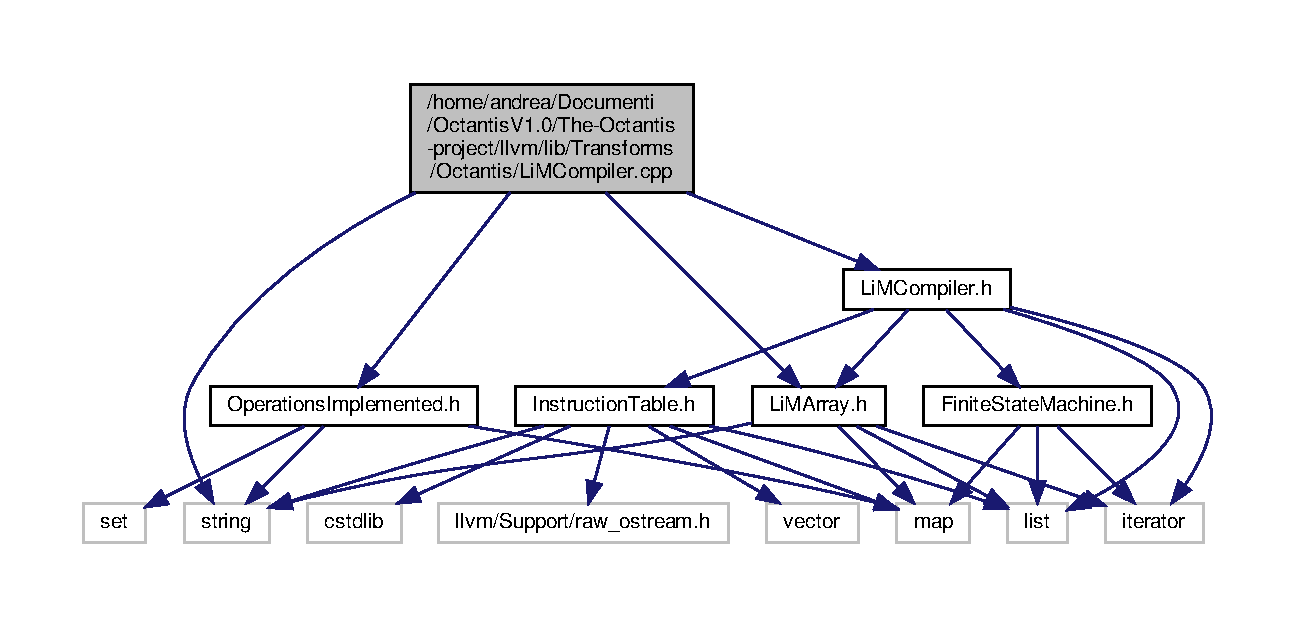
\includegraphics[width=350pt]{LiMCompiler_8cpp__incl}
\end{center}
\end{figure}

\hypertarget{LiMCompiler_8h}{}\section{/home/andrea/\+Documenti/\+Octantis\+V1.0/\+The-\/\+Octantis-\/project/llvm/lib/\+Transforms/\+Octantis/\+Li\+M\+Compiler.h File Reference}
\label{LiMCompiler_8h}\index{/home/andrea/\+Documenti/\+Octantis\+V1.\+0/\+The-\/\+Octantis-\/project/llvm/lib/\+Transforms/\+Octantis/\+Li\+M\+Compiler.\+h@{/home/andrea/\+Documenti/\+Octantis\+V1.\+0/\+The-\/\+Octantis-\/project/llvm/lib/\+Transforms/\+Octantis/\+Li\+M\+Compiler.\+h}}
{\ttfamily \#include \char`\"{}Instruction\+Table.\+h\char`\"{}}\newline
{\ttfamily \#include \char`\"{}Li\+M\+Array.\+h\char`\"{}}\newline
{\ttfamily \#include \char`\"{}Finite\+State\+Machine.\+h\char`\"{}}\newline
{\ttfamily \#include $<$list$>$}\newline
{\ttfamily \#include $<$iterator$>$}\newline
Include dependency graph for Li\+M\+Compiler.\+h\+:
\nopagebreak
\begin{figure}[H]
\begin{center}
\leavevmode
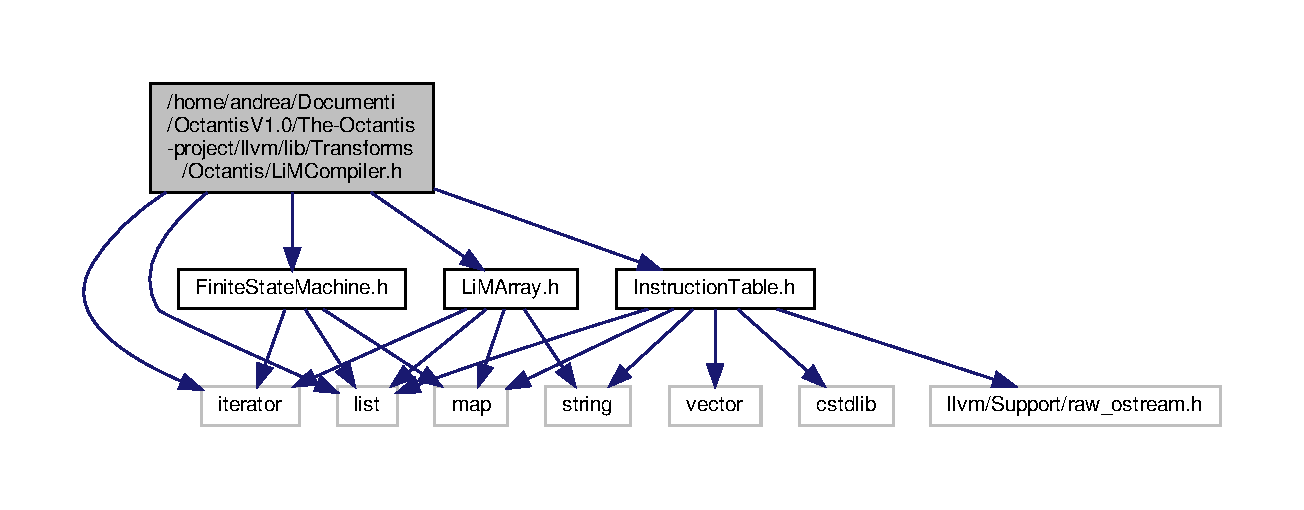
\includegraphics[width=350pt]{LiMCompiler_8h__incl}
\end{center}
\end{figure}
This graph shows which files directly or indirectly include this file\+:
\nopagebreak
\begin{figure}[H]
\begin{center}
\leavevmode
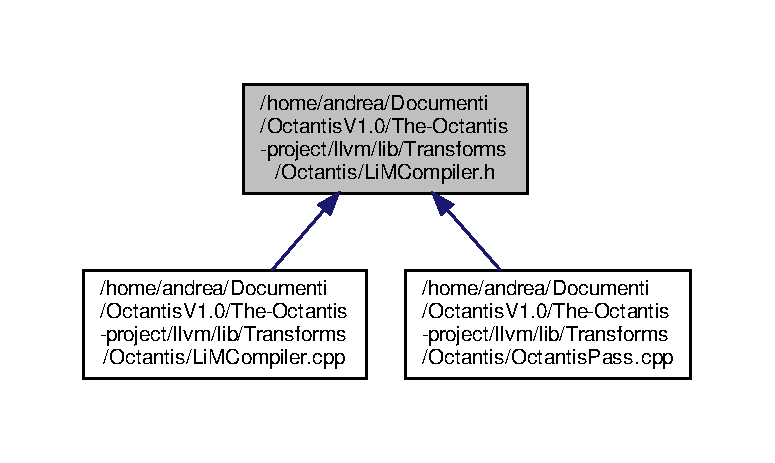
\includegraphics[width=350pt]{LiMCompiler_8h__dep__incl}
\end{center}
\end{figure}
\subsection*{Classes}
\begin{DoxyCompactItemize}
\item 
class \hyperlink{classoctantis_1_1LiMCompiler}{octantis\+::\+Li\+M\+Compiler}
\begin{DoxyCompactList}\small\item\em Class class useful for the generation of a LiM object. \end{DoxyCompactList}\end{DoxyCompactItemize}
\subsection*{Namespaces}
\begin{DoxyCompactItemize}
\item 
 \hyperlink{namespaceoctantis}{octantis}
\end{DoxyCompactItemize}

\hypertarget{OctantisPass_8cpp}{}\section{/home/andrea/\+Documenti/\+Octantis\+V1.0/\+The-\/\+Octantis-\/project/llvm/lib/\+Transforms/\+Octantis/\+Octantis\+Pass.cpp File Reference}
\label{OctantisPass_8cpp}\index{/home/andrea/\+Documenti/\+Octantis\+V1.\+0/\+The-\/\+Octantis-\/project/llvm/lib/\+Transforms/\+Octantis/\+Octantis\+Pass.\+cpp@{/home/andrea/\+Documenti/\+Octantis\+V1.\+0/\+The-\/\+Octantis-\/project/llvm/lib/\+Transforms/\+Octantis/\+Octantis\+Pass.\+cpp}}
{\ttfamily \#include \char`\"{}llvm/\+A\+D\+T/\+Statistic.\+h\char`\"{}}\newline
{\ttfamily \#include \char`\"{}llvm/\+I\+R/\+Function.\+h\char`\"{}}\newline
{\ttfamily \#include \char`\"{}llvm/\+Pass.\+h\char`\"{}}\newline
{\ttfamily \#include \char`\"{}llvm/\+Support/raw\+\_\+ostream.\+h\char`\"{}}\newline
{\ttfamily \#include \char`\"{}llvm/\+I\+R/\+User.\+h\char`\"{}}\newline
{\ttfamily \#include \char`\"{}llvm/\+Analysis/\+Dependence\+Analysis.\+h\char`\"{}}\newline
{\ttfamily \#include \char`\"{}Scheduling\+A\+S\+A\+P.\+h\char`\"{}}\newline
{\ttfamily \#include \char`\"{}Li\+M\+Compiler.\+h\char`\"{}}\newline
Include dependency graph for Octantis\+Pass.\+cpp\+:
% FIG 0
\subsection*{Classes}
\begin{DoxyCompactItemize}
\item 
struct \hyperlink{structoctantis_1_1OctantisPass}{octantis\+::\+Octantis\+Pass}
\end{DoxyCompactItemize}
\subsection*{Namespaces}
\begin{DoxyCompactItemize}
\item 
 \hyperlink{namespaceoctantis}{octantis}
\end{DoxyCompactItemize}


\subsection{Detailed Description}
Octantis\+Pass Pass\+: backend pass for the generation of Dexima\textquotesingle{}s configuration files. 
\hypertarget{OperationsImplemented_8h}{}\section{/home/andrea/\+Documenti/\+Octantis\+V1.0/\+The-\/\+Octantis-\/project/llvm/lib/\+Transforms/\+Octantis/\+Operations\+Implemented.h File Reference}
\label{OperationsImplemented_8h}\index{/home/andrea/\+Documenti/\+Octantis\+V1.\+0/\+The-\/\+Octantis-\/project/llvm/lib/\+Transforms/\+Octantis/\+Operations\+Implemented.\+h@{/home/andrea/\+Documenti/\+Octantis\+V1.\+0/\+The-\/\+Octantis-\/project/llvm/lib/\+Transforms/\+Octantis/\+Operations\+Implemented.\+h}}
{\ttfamily \#include $<$string$>$}\newline
{\ttfamily \#include $<$map$>$}\newline
{\ttfamily \#include $<$set$>$}\newline
Include dependency graph for Operations\+Implemented.\+h\+:
\nopagebreak
\begin{figure}[H]
\begin{center}
\leavevmode
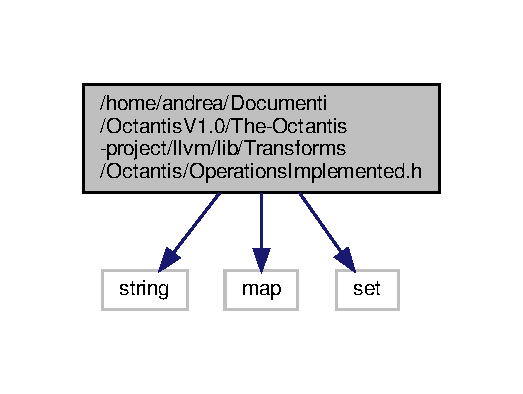
\includegraphics[width=251pt]{OperationsImplemented_8h__incl}
\end{center}
\end{figure}
This graph shows which files directly or indirectly include this file\+:
\nopagebreak
\begin{figure}[H]
\begin{center}
\leavevmode
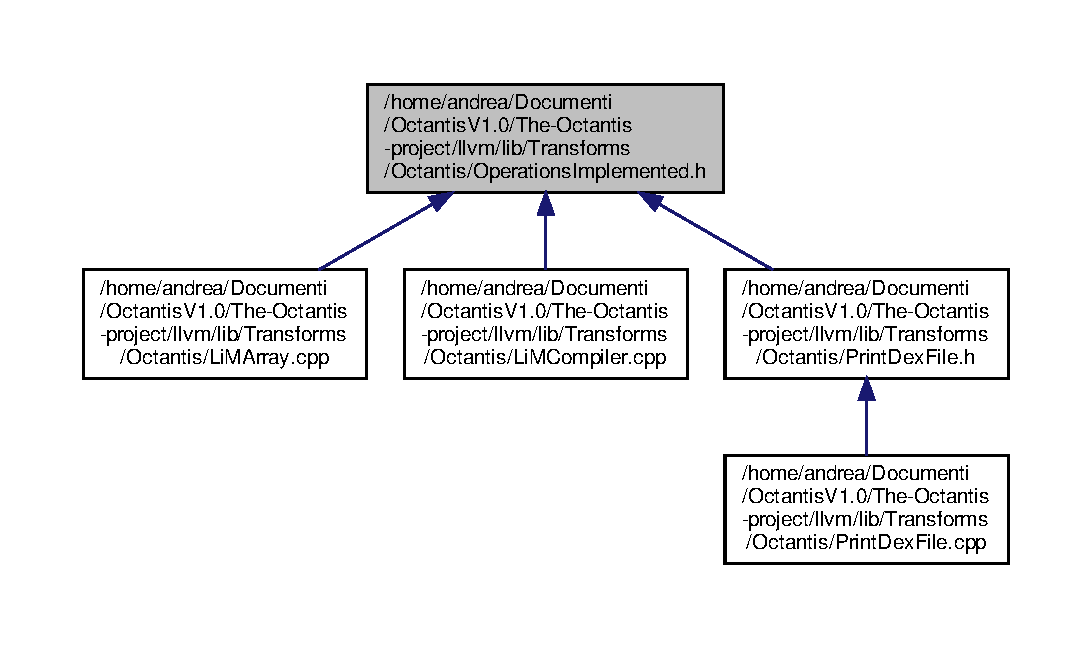
\includegraphics[width=350pt]{OperationsImplemented_8h__dep__incl}
\end{center}
\end{figure}
\subsection*{Namespaces}
\begin{DoxyCompactItemize}
\item 
 \hyperlink{namespaceoctantis}{octantis}
\end{DoxyCompactItemize}
\subsection*{Variables}
\begin{DoxyCompactItemize}
\item 
const std\+::map$<$ std\+::string, std\+::string $>$ \hyperlink{namespaceoctantis_a49f0001417908900d6959ac7a8037ebd}{octantis\+::\+Lim\+Operations}
\item 
const std\+::set$<$ std\+::string $>$ \hyperlink{namespaceoctantis_adec74f4b9921d5c7eecef4f9174c3510}{octantis\+::\+Periperal\+Operations}
\end{DoxyCompactItemize}


\subsection{Detailed Description}
Operations Implemented Include File\+: it includes all the macto-\/operations recognized by D\+Ex\+I\+MA 
\hypertarget{PrintDexFile_8cpp}{}\section{/home/andrea/\+Documenti/\+Octantis\+V1.0/\+The-\/\+Octantis-\/project/llvm/lib/\+Transforms/\+Octantis/\+Print\+Dex\+File.cpp File Reference}
\label{PrintDexFile_8cpp}\index{/home/andrea/\+Documenti/\+Octantis\+V1.\+0/\+The-\/\+Octantis-\/project/llvm/lib/\+Transforms/\+Octantis/\+Print\+Dex\+File.\+cpp@{/home/andrea/\+Documenti/\+Octantis\+V1.\+0/\+The-\/\+Octantis-\/project/llvm/lib/\+Transforms/\+Octantis/\+Print\+Dex\+File.\+cpp}}
{\ttfamily \#include \char`\"{}Print\+Dex\+File.\+h\char`\"{}}\newline
{\ttfamily \#include $<$cmath$>$}\newline
Include dependency graph for Print\+Dex\+File.\+cpp\+:
% FIG 0

\hypertarget{PrintDexFile_8h}{}\section{/home/andrea/\+Documenti/\+Octantis\+V1.0/\+The-\/\+Octantis-\/project/llvm/lib/\+Transforms/\+Octantis/\+Print\+Dex\+File.h File Reference}
\label{PrintDexFile_8h}\index{/home/andrea/\+Documenti/\+Octantis\+V1.\+0/\+The-\/\+Octantis-\/project/llvm/lib/\+Transforms/\+Octantis/\+Print\+Dex\+File.\+h@{/home/andrea/\+Documenti/\+Octantis\+V1.\+0/\+The-\/\+Octantis-\/project/llvm/lib/\+Transforms/\+Octantis/\+Print\+Dex\+File.\+h}}
{\ttfamily \#include \char`\"{}llvm/\+Support/raw\+\_\+ostream.\+h\char`\"{}}\newline
{\ttfamily \#include \char`\"{}Finite\+State\+Machine.\+h\char`\"{}}\newline
{\ttfamily \#include \char`\"{}Operations\+Implemented.\+h\char`\"{}}\newline
{\ttfamily \#include \char`\"{}Li\+M\+Array.\+h\char`\"{}}\newline
{\ttfamily \#include $<$sstream$>$}\newline
{\ttfamily \#include $<$map$>$}\newline
{\ttfamily \#include $<$string$>$}\newline
{\ttfamily \#include $<$iterator$>$}\newline
{\ttfamily \#include $<$set$>$}\newline
Include dependency graph for Print\+Dex\+File.\+h\+:
\nopagebreak
\begin{figure}[H]
\begin{center}
\leavevmode
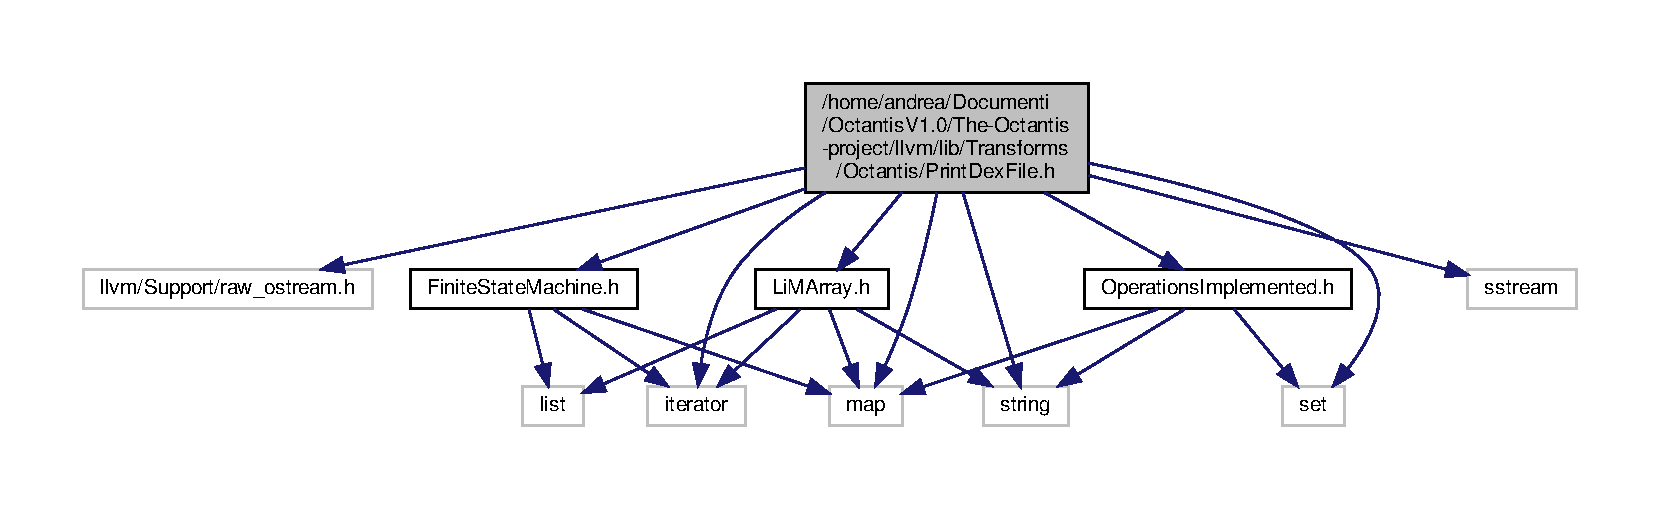
\includegraphics[width=350pt]{PrintDexFile_8h__incl}
\end{center}
\end{figure}
This graph shows which files directly or indirectly include this file\+:
\nopagebreak
\begin{figure}[H]
\begin{center}
\leavevmode
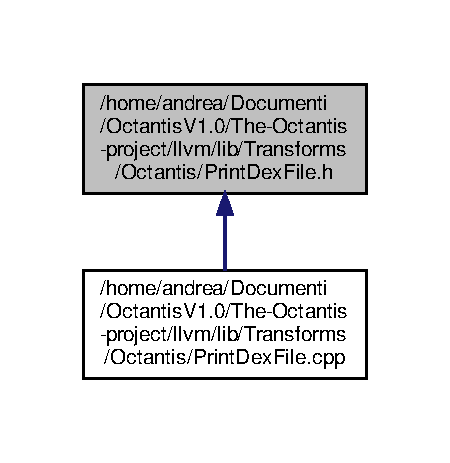
\includegraphics[width=216pt]{PrintDexFile_8h__dep__incl}
\end{center}
\end{figure}
\subsection*{Classes}
\begin{DoxyCompactItemize}
\item 
class \hyperlink{classoctantis_1_1PrintDexFile}{octantis\+::\+Print\+Dex\+File}
\begin{DoxyCompactList}\small\item\em Class class useful for the definition of Dexima\textquotesingle{}s configuration file (.dex). \end{DoxyCompactList}\end{DoxyCompactItemize}
\subsection*{Namespaces}
\begin{DoxyCompactItemize}
\item 
 \hyperlink{namespaceoctantis}{octantis}
\end{DoxyCompactItemize}

\hypertarget{SchedulingASAP_8cpp}{}\section{/home/andrea/\+Documenti/\+Octantis\+V1.0/\+The-\/\+Octantis-\/project/llvm/lib/\+Transforms/\+Octantis/\+Scheduling\+A\+S\+AP.cpp File Reference}
\label{SchedulingASAP_8cpp}\index{/home/andrea/\+Documenti/\+Octantis\+V1.\+0/\+The-\/\+Octantis-\/project/llvm/lib/\+Transforms/\+Octantis/\+Scheduling\+A\+S\+A\+P.\+cpp@{/home/andrea/\+Documenti/\+Octantis\+V1.\+0/\+The-\/\+Octantis-\/project/llvm/lib/\+Transforms/\+Octantis/\+Scheduling\+A\+S\+A\+P.\+cpp}}
{\ttfamily \#include \char`\"{}Scheduling\+A\+S\+A\+P.\+h\char`\"{}}\newline
{\ttfamily \#include \char`\"{}llvm/\+I\+R/\+Function.\+h\char`\"{}}\newline
{\ttfamily \#include \char`\"{}llvm/\+I\+R/\+Module.\+h\char`\"{}}\newline
{\ttfamily \#include \char`\"{}llvm/\+I\+R/\+Instructions.\+h\char`\"{}}\newline
{\ttfamily \#include \char`\"{}llvm/\+Support/raw\+\_\+ostream.\+h\char`\"{}}\newline
{\ttfamily \#include \char`\"{}llvm/\+I\+R/\+User.\+h\char`\"{}}\newline
{\ttfamily \#include \char`\"{}llvm/\+Bitstream/\+Bit\+Codes.\+h\char`\"{}}\newline
{\ttfamily \#include $<$string$>$}\newline
{\ttfamily \#include $<$algorithm$>$}\newline
Include dependency graph for Scheduling\+A\+S\+A\+P.\+cpp\+:
% FIG 0

\hypertarget{SchedulingASAP_8h}{}\section{/home/andrea/\+Documenti/\+Octantis\+V1.0/\+The-\/\+Octantis-\/project/llvm/lib/\+Transforms/\+Octantis/\+Scheduling\+A\+S\+AP.h File Reference}
\label{SchedulingASAP_8h}\index{/home/andrea/\+Documenti/\+Octantis\+V1.\+0/\+The-\/\+Octantis-\/project/llvm/lib/\+Transforms/\+Octantis/\+Scheduling\+A\+S\+A\+P.\+h@{/home/andrea/\+Documenti/\+Octantis\+V1.\+0/\+The-\/\+Octantis-\/project/llvm/lib/\+Transforms/\+Octantis/\+Scheduling\+A\+S\+A\+P.\+h}}
{\ttfamily \#include \char`\"{}llvm/\+I\+R/\+Function.\+h\char`\"{}}\newline
{\ttfamily \#include \char`\"{}Instruction\+Table.\+h\char`\"{}}\newline
{\ttfamily \#include $<$map$>$}\newline
{\ttfamily \#include $<$iterator$>$}\newline
Include dependency graph for Scheduling\+A\+S\+A\+P.\+h\+:
% FIG 0
This graph shows which files directly or indirectly include this file\+:
% FIG 1
\subsection*{Classes}
\begin{DoxyCompactItemize}
\item 
class \hyperlink{classoctantis_1_1SchedulingASAP}{octantis\+::\+Scheduling\+A\+S\+AP}
\begin{DoxyCompactList}\small\item\em Class useful for the implementation of the A\+S\+AP Scheduling algorithm. \end{DoxyCompactList}\end{DoxyCompactItemize}
\subsection*{Namespaces}
\begin{DoxyCompactItemize}
\item 
 \hyperlink{namespaceoctantis}{octantis}
\end{DoxyCompactItemize}

%--- End generated contents ---

% Index
\backmatter
\newpage
\phantomsection
\clearemptydoublepage
\addcontentsline{toc}{chapter}{Index}
\printindex

\end{document}
